\RequirePackage{fix-cm}
\documentclass[12pt,letterpaper]{article}
\usepackage[margin=1in,headheight=15pt,headsep=15pt]{geometry}
\usepackage{amsmath,amssymb,graphicx,booktabs,array,float,fancyhdr,lastpage,hyperref,listings,xcolor}
\usepackage{microtype,needspace,fontspec,placeins}
\usepackage{capt-of}
\usepackage{subcaption}
\captionsetup[subfigure]{font=normalsize,labelfont=bf,justification=centering}
\usepackage{tikz}
\usetikzlibrary{arrows.meta}
\setmainfont{Times New Roman}
\setlength{\emergencystretch}{2em}
\hypersetup{colorlinks=false,hidelinks}
\pagestyle{fancy}\fancyhf{}
\fancyhead[L]{\normalsize Problem B}
\fancyhead[C]{\small The University Physics Competition}
\fancyhead[R]{\small Page \thepage\ of \pageref{LastPage}}
\renewcommand{\headrulewidth}{0.4pt}
\setlength{\parindent}{1.5em}
\setlength{\parskip}{0pt}
\lstset{basicstyle=\ttfamily\footnotesize,breaklines=true,numbers=left,numberstyle=\tiny,numbersep=8pt,columns=fullflexible,showstringspaces=false,frame=none}
\graphicspath{{aerodynamics/}{assets/}{../results/current_report/figures/}{../results/sensitivity_linear/figures/}}

% BEGIN REPORT_RESULTS
% Generated exclusively from results/current_report.
\newcommand{\WMXMOneGoalError}{---}
\newcommand{\WMXMOnePathRMSE}{0.244}
\newcommand{\WMXMOneEarlyResidual}{36.00}
\newcommand{\WMXMTwoGoalError}{---}
\newcommand{\WMXMTwoPathRMSE}{0.136}
\newcommand{\WMXMTwoEarlyResidual}{26.13}
\newcommand{\WMXMThreeGoalError}{---}
\newcommand{\WMXMThreePathRMSE}{0.826}
\newcommand{\WMXMThreeEarlyResidual}{0.00}
\newcommand{\WMXMFourGoalError}{0.360}
\newcommand{\WMXMFourPathRMSE}{0.234}
\newcommand{\WMXMFourEarlyResidual}{25.90}
\newcommand{\WMXSpeed}{29.20}
\newcommand{\WMXDrag}{7.05}
\newcommand{\WMXCD}{0.3623}
\newcommand{\WMXAlpha}{2.2877}
\newcommand{\WOHMOneGoalError}{0.684}
\newcommand{\WOHMOnePathRMSE}{0.412}
\newcommand{\WOHMOneEarlyResidual}{12.00}
\newcommand{\WOHMTwoGoalError}{0.657}
\newcommand{\WOHMTwoPathRMSE}{0.356}
\newcommand{\WOHMTwoEarlyResidual}{10.28}
\newcommand{\WOHMThreeGoalError}{0.374}
\newcommand{\WOHMThreePathRMSE}{0.190}
\newcommand{\WOHMThreeEarlyResidual}{0.00}
\newcommand{\WOHMFourGoalError}{0.113}
\newcommand{\WOHMFourPathRMSE}{0.093}
\newcommand{\WOHMFourEarlyResidual}{2.90}
\newcommand{\WOHSpeed}{32.05}
\newcommand{\WOHDrag}{7.58}
\newcommand{\WOHCD}{0.3238}
\newcommand{\WOHAlpha}{2.2877}
\newcommand{\WRMOneGoalError}{0.475}
\newcommand{\WRMOnePathRMSE}{0.300}
\newcommand{\WRMOneEarlyResidual}{8.00}
\newcommand{\WRMTwoGoalError}{0.475}
\newcommand{\WRMTwoPathRMSE}{0.320}
\newcommand{\WRMTwoEarlyResidual}{7.01}
\newcommand{\WRMThreeGoalError}{0.155}
\newcommand{\WRMThreePathRMSE}{0.151}
\newcommand{\WRMThreeEarlyResidual}{0.00}
\newcommand{\WRMFourGoalError}{0.146}
\newcommand{\WRMFourPathRMSE}{0.132}
\newcommand{\WRMFourEarlyResidual}{1.12}
\newcommand{\WRSpeed}{28.34}
\newcommand{\WRDrag}{2.21}
\newcommand{\WRCD}{0.1208}
\newcommand{\WRAlpha}{2.2877}
\newcommand{\PenaltyErrorSummaryTable}{\begin{table}[H]\centering\normalfont\normalsize
\renewcommand{\arraystretch}{1.12}
\caption{Early maximum coordinate residual, subsequent path RMSE/sample count, goal-plane error and termination.}\label{tab:penalty-errors}
\setlength{\tabcolsep}{4pt}\begin{tabular}{llrrrl}\toprule
Event & Model & Residual (mm) & RMSE (m)/$n$ & Goal (m) & Status\\\midrule
Placement 1 & M1 & 36.00 & 0.244/3 & --- & ground\\
Placement 1 & M2 & 26.13 & 0.136/3 & --- & ground\\
Placement 1 & M3 & 0.00 & 0.826/6 & --- & no crossing\\
Placement 1 & M4 & 25.90 & 0.234/5 & 0.360 & goal\\
Power shot & M1 & 12.00 & 0.412/6 & 0.684 & goal\\
Power shot & M2 & 10.28 & 0.356/7 & 0.657 & goal\\
Power shot & M3 & 0.00 & 0.190/7 & 0.374 & goal\\
Power shot & M4 & 2.90 & 0.093/7 & 0.113 & goal\\
Placement 2 & M1 & 8.00 & 0.300/5 & 0.475 & goal\\
Placement 2 & M2 & 7.01 & 0.320/6 & 0.475 & goal\\
Placement 2 & M3 & 0.00 & 0.151/5 & 0.155 & goal\\
Placement 2 & M4 & 1.12 & 0.132/5 & 0.146 & goal\\
\bottomrule\end{tabular}\end{table}}
\newcommand{\WMXMThreeMaxX}{10.973}
\newcommand{\MFourParameterTable}{\begin{table}[H]\centering\small
\caption{Fitted M4 states at the selected starting frames.}\label{tab:m4-parameters}
\setlength{\tabcolsep}{4pt}\begin{tabular}{lrrrrrr}\toprule
Event & $v_0$ (m/s) & $C_D$ & $\alpha$ & $n_x$ & $n_y$ & $n_z$\\\midrule
J03WMX & 29.20 & 0.3623 & 2.2877 & 0.2280 & -0.9728 & 0.0413\\
J03WR9 & 28.34 & 0.1208 & 2.2877 & 0.1439 & -0.2711 & -0.9517\\
J03WOH & 32.05 & 0.3238 & 2.2877 & -0.2276 & 0.3170 & 0.9207\\
\bottomrule\end{tabular}\end{table}}
\newcommand{\ReferenceCD}{0.2415}
\newcommand{\ReferenceCL}{1.5251}
\newcommand{\ForwardReMin}{2.05}
\newcommand{\ForwardReMax}{3.96}
\newcommand{\CurvedY}{0.8415}
\newcommand{\CurvedZ}{0.8769}
\newcommand{\CurvedTime}{0.5022}
\newcommand{\CurvedVX}{23.6354}
\newcommand{\CurvedVZ}{4.1676}
\newcommand{\PenaltyInputsTable}{\begin{table}[H]\centering\footnotesize
\caption{Frame counts, fitting times and measured local starting positions.}\label{tab:penalty-inputs}
\setlength{\tabcolsep}{4pt}\begin{tabular}{lrrl}\toprule
Event & Frames & Fit times (s) & $\boldsymbol r_0$ (m)\\\midrule
J03WMX & 15 & 0.00,0.04,0.08 & $(3.04,0.55,0.13)$\\
J03WOH & 12 & 0.00,0.04,0.08 & $(0.77,0.08,0.24)$\\
J03WR9 & 12 & 0.00,0.04,0.08 & $(2.57,0.85,0.34)$\\
\bottomrule\end{tabular}\end{table}}
\newcommand{\PenaltyObservationTable}{\begin{table}[H]\centering\small
\caption{Selected early positions and observed goal crossings in local coordinates.}\label{tab:penalty-observations}
\setlength{\tabcolsep}{4pt}\begin{tabular}{llrrrr}\toprule
Event & Source frame & $t$ (s) & $x$ (m) & $y$ (m) & $z$ (m)\\\midrule
Placement 1 & 152602 & 0.00 & 3.040 & 0.550 & 0.130\\
Placement 1 & 152603 & 0.04 & 4.190 & 0.820 & 0.150\\
Placement 1 & 152604 & 0.08 & 5.250 & 1.070 & 0.180\\
Placement 1 goal & 152610 & 0.3200 & 11.0000 & 2.7500 & 0.1600\\
Placement 2 & 176245 & 0.00 & 2.570 & 0.850 & 0.340\\
Placement 2 & 176246 & 0.04 & 3.640 & 1.200 & 0.410\\
Placement 2 & 176247 & 0.08 & 4.710 & 1.530 & 0.470\\
Placement 2 goal & 176253--176254 & 0.3295 & 11.0000 & 3.0697 & 0.4657\\
Power shot & 128955 & 0.00 & 0.770 & 0.080 & 0.240\\
Power shot & 128956 & 0.04 & 1.990 & 0.340 & 0.460\\
Power shot & 128957 & 0.08 & 3.180 & 0.620 & 0.650\\
Power shot goal & 128964--128965 & 0.3643 & 11.0000 & 2.9188 & 1.1789\\
\bottomrule\end{tabular}\end{table}}
\newcommand{\InverseBoundsTable}{\begin{table}[H]\centering\footnotesize
\caption{Component bounds and force-correction settings for inversion.}\label{tab:inverse-bounds}
\setlength{\tabcolsep}{4pt}\begin{tabular}{ll}\toprule
Quantity & Search interval\\\midrule
$v_{x0}$ (M1, M2, M4) & $[0,35]$ m/s\\
$v_{y0},v_{z0}$ (M1, M2, M4) & $[-35,35]$ m/s\\
$\|\boldsymbol\omega_0\|$ (M4) & $30$ rad/s\\
Azimuth, elevation (M4) & $[-\pi,\pi],[-\pi/2,\pi/2]$ rad\\
$C_D/C_D^*,\alpha/\alpha^*$ & $[0.5,1.5]$\\
\bottomrule\end{tabular}\end{table}}
\newcommand{\WMXMeasuredTable}{\begin{table}[H]\centering\footnotesize
\caption{J03WMX: three measured fitting points and observed goal crossing (direct source frame).}\label{tab:measured-J03WMX}
\setlength{\tabcolsep}{4pt}\begin{tabular}{llrrrr}\toprule
Point & Source frame & $t$ (s) & $x$ (m) & $y$ (m) & $z$ (m)\\\midrule
$P_0$ & 152602 & 0.00 & 3.040 & 0.550 & 0.130\\
$P_1$ & 152603 & 0.04 & 4.190 & 0.820 & 0.150\\
$P_2$ & 152604 & 0.08 & 5.250 & 1.070 & 0.180\\
Goal & 152610 & 0.3200 & 11.000 & 2.7500 & 0.1600\\
\bottomrule\end{tabular}\end{table}}
\newcommand{\WMXPredictedTable}{\begin{table}[H]\centering\footnotesize
\caption{J03WMX: inverse initial states and predicted goal-plane crossings. M4 uses a 30 rad/s reference spin magnitude; M1--M3 do not estimate spin.}\label{tab:predicted-J03WMX}
\setlength{\tabcolsep}{4pt}\begin{tabular}{llrrccr}\toprule
Model & Status & $y_g$ (m) & $z_g$ (m) & $\boldsymbol v_0$ (m/s) & Spin & $d_g$ (m)\\\midrule
M1 & ground & --- & --- & $\begin{pmatrix}27.850\\6.550\\0.953\end{pmatrix}$ & --- & ---\\
M2 & ground & --- & --- & $\begin{pmatrix}28.411\\6.682\\0.967\end{pmatrix}$ & --- & ---\\
M3 & time limit & --- & --- & $\begin{pmatrix}29.875\\7.000\\0.375\end{pmatrix}$ & --- & ---\\
M4 & plane & 2.4377 & 0.3390 & $\begin{pmatrix}28.423\\6.667\\0.551\end{pmatrix}$ & $\begin{pmatrix}6.839\\-29.184\\1.239\end{pmatrix}$ & 0.3600\\
\bottomrule\end{tabular}\end{table}}
\newcommand{\WMXDiscussion}{The measured low flight requires sustained vertical support from lift. M4's crossing deviation is 0.3600 m. Ground contact precedes the goal for M1, M2.}
\newcommand{\WOHMeasuredTable}{\begin{table}[H]\centering\footnotesize
\caption{J03WOH: three measured fitting points and observed goal crossing (linear interpolation).}\label{tab:measured-J03WOH}
\setlength{\tabcolsep}{4pt}\begin{tabular}{llrrrr}\toprule
Point & Source frame & $t$ (s) & $x$ (m) & $y$ (m) & $z$ (m)\\\midrule
$P_0$ & 128955 & 0.00 & 0.770 & 0.080 & 0.240\\
$P_1$ & 128956 & 0.04 & 1.990 & 0.340 & 0.460\\
$P_2$ & 128957 & 0.08 & 3.180 & 0.620 & 0.650\\
Goal & 128964--128965 & 0.3643 & 11.000 & 2.9188 & 1.1789\\
\bottomrule\end{tabular}\end{table}}
\newcommand{\WOHPredictedTable}{\begin{table}[H]\centering\footnotesize
\caption{J03WOH: inverse initial states and predicted goal-plane crossings. M4 uses a 30 rad/s reference spin magnitude; M1--M3 do not estimate spin.}\label{tab:predicted-J03WOH}
\setlength{\tabcolsep}{4pt}\begin{tabular}{llrrccr}\toprule
Model & Status & $y_g$ (m) & $z_g$ (m) & $\boldsymbol v_0$ (m/s) & Spin & $d_g$ (m)\\\midrule
M1 & plane & 2.3496 & 1.5583 & $\begin{pmatrix}30.200\\6.700\\5.553\end{pmatrix}$ & --- & 0.6841\\
M2 & plane & 2.3494 & 1.5059 & $\begin{pmatrix}30.794\\6.831\\5.658\end{pmatrix}$ & --- & 0.6567\\
M3 & plane & 3.2890 & 1.1262 & $\begin{pmatrix}30.875\\6.250\\5.875\end{pmatrix}$ & --- & 0.3739\\
M4 & plane & 2.9344 & 1.2906 & $\begin{pmatrix}30.857\\6.408\\5.819\end{pmatrix}$ & $\begin{pmatrix}-6.829\\9.510\\27.621\end{pmatrix}$ & 0.1127\\
\bottomrule\end{tabular}\end{table}}
\newcommand{\WOHDiscussion}{The rising measured arc connects vertical launch velocity with the subsequent action of gravity and lift. M4's crossing deviation is 0.1127 m.}
\newcommand{\WRMeasuredTable}{\begin{table}[H]\centering\footnotesize
\caption{J03WR9: three measured fitting points and observed goal crossing (linear interpolation).}\label{tab:measured-J03WR9}
\setlength{\tabcolsep}{4pt}\begin{tabular}{llrrrr}\toprule
Point & Source frame & $t$ (s) & $x$ (m) & $y$ (m) & $z$ (m)\\\midrule
$P_0$ & 176245 & 0.00 & 2.570 & 0.850 & 0.340\\
$P_1$ & 176246 & 0.04 & 3.640 & 1.200 & 0.410\\
$P_2$ & 176247 & 0.08 & 4.710 & 1.530 & 0.470\\
Goal & 176253--176254 & 0.3295 & 11.000 & 3.0697 & 0.4657\\
\bottomrule\end{tabular}\end{table}}
\newcommand{\WRPredictedTable}{\begin{table}[H]\centering\footnotesize
\caption{J03WR9: inverse initial states and predicted goal-plane crossings. M4 uses a 30 rad/s reference spin magnitude; M1--M3 do not estimate spin.}\label{tab:predicted-J03WR9}
\setlength{\tabcolsep}{4pt}\begin{tabular}{llrrccr}\toprule
Model & Status & $y_g$ (m) & $z_g$ (m) & $\boldsymbol v_0$ (m/s) & Spin & $d_g$ (m)\\\midrule
M1 & plane & 3.5444 & 0.4841 & $\begin{pmatrix}26.750\\8.550\\2.003\end{pmatrix}$ & --- & 0.4751\\
M2 & plane & 3.5445 & 0.4712 & $\begin{pmatrix}26.924\\8.606\\2.015\end{pmatrix}$ & --- & 0.4749\\
M3 & plane & 3.0656 & 0.6205 & $\begin{pmatrix}26.750\\9.000\\1.875\end{pmatrix}$ & --- & 0.1549\\
M4 & plane & 3.1189 & 0.6035 & $\begin{pmatrix}26.812\\8.977\\1.892\end{pmatrix}$ & $\begin{pmatrix}4.317\\-8.132\\-28.552\end{pmatrix}$ & 0.1463\\
\bottomrule\end{tabular}\end{table}}
\newcommand{\WRDiscussion}{The measured path bends laterally, so fitted spin direction affects the continuation towards the goal. M4's crossing deviation is 0.1463 m.}
\newcommand{\TorqueViscousRatio}{$3.54\times10^{-4}$}
\newcommand{\TorqueDisplacement}{0.0616}
\newcommand{\TorqueResults}{Spin falls by 19.740\%, while the crossing moves 0.0616 m (0.560\% of the 11 m distance) and arrival time changes by -0.066\%. Rotational damping therefore has a small endpoint effect in this short reference flight.}
\newcommand{\WindResultsTable}{\begin{table}[H]\centering\footnotesize
\caption{Illustrative wind at the 24 m/s curved-shot launch: dynamic-pressure changes at fixed coefficients.}\label{tab:wind}
\setlength{\tabcolsep}{4pt}\begin{tabular}{rrrrr}\toprule
$w$ (m/s) & Headwind (\%) & Tailwind (\%) & Crosswind (\%) & Angle ($^\circ$)\\\midrule
1 & +8.51 & -8.16 & +0.17 & 2.39\\
3 & +26.56 & -23.44 & +1.56 & 7.13\\
5 & +46.01 & -37.33 & +4.34 & 11.77\\
\bottomrule\end{tabular}\end{table}}
\newcommand{\WindThreshold}{0.59}
% END REPORT_RESULTS

% BEGIN SENSITIVITY_RESULTS
% Generated from reviewed sensitivity data; keep mass and radius fixed.
\newcommand{\SensitivityFixedRuns}{369}
\newcommand{\SensitivityMaxDirection}{20.218}
\newcommand{\SensitivityConditionalShift}{0.1074}
\newcommand{\SensitivityConditionalResidual}{1.86\times10^{-3}}
\newcommand{\MCCount}{100000}
\newcommand{\MCSeed}{20261108}
\newcommand{\MCMeanY}{2.6170}
\newcommand{\MCMeanZ}{1.9511}
\newcommand{\MCStdY}{0.2455}
\newcommand{\MCStdZ}{0.2360}
\newcommand{\MCMaxDisplacement}{0.801}
\newcommand{\MCClearCount}{95772}
\newcommand{\MCOverCount}{4228}
\newcommand{\MCClearPercent}{95.772}
\newcommand{\MCOverPercent}{4.228}
\newcommand{\MCJointThreshold}{4.5916}
\newcommand{\MCAdaptiveError}{1.19\times10^{-12}}
\newcommand{\MCHalfStepError}{1.43\times10^{-12}}
\newcommand{\MCCheckCount}{70}
\newcommand{\SensitivityReferenceVX}{30.3784}
\newcommand{\SensitivityReferenceVY}{9.4074}
\newcommand{\SensitivityReferenceVZ}{6.8974}
\newcommand{\SensitivityReferenceWX}{19.7434}
\newcommand{\SensitivityReferenceWY}{1.2060}
\newcommand{\SensitivityReferenceWZ}{-22.5553}
\newcommand{\SensitivityReferenceCD}{0.3623}
\newcommand{\SensitivityReferenceAlpha}{2.2877}
\newcommand{\SensitivityReferenceY}{2.6159}
\newcommand{\SensitivityReferenceZ}{1.9526}
\newcommand{\SensitivityReferenceTime}{0.398967}
\newcommand{\SensitivityReferenceResidual}{0.784}
\newcommand{\SensitivityWideCount}{5049}
\newcommand{\SensitivityInnerCount}{2079}
\newcommand{\MCDisplayClear}{385}
\newcommand{\MCDisplayHigh}{15}
\newcommand{\SensitivitySpeedShift}{8.356}
\newcommand{\SensitivitySpeedTime}{20.659}
\newcommand{\SensitivityYawShift}{20.070}
\newcommand{\SensitivityYawTime}{1.965}
\newcommand{\SensitivityPitchShift}{20.218}
\newcommand{\SensitivityPitchTime}{1.692}
\newcommand{\SensitivitySpinShift}{3.873}
\newcommand{\SensitivitySpinTime}{0.287}
\newcommand{\SensitivityDragShift}{0.620}
\newcommand{\SensitivityDragTime}{2.274}
\newcommand{\SensitivityLiftShift}{3.873}
\newcommand{\SensitivityLiftTime}{0.287}
\newcommand{\MCReplicaY}{5.425}
\newcommand{\MCConvergenceY}{0.264}
\newcommand{\MCReplicaZ}{4.320}
\newcommand{\MCConvergenceZ}{0.506}
\newcommand{\MCReplicaT}{0.328}
\newcommand{\MCConvergenceT}{0.138}
\newcommand{\SensitivityOneFactorTable}{\begin{table}[H]\centering\small
\caption{Goal-plane displacement and arrival-time change under one-factor perturbations.}\label{tab:sensitivity-one-factor}
\begin{tabular}{p{.32\textwidth}crr}\toprule
Parameter & Perturbation & $\max D_g$ (cm) & $\max|\Delta t_g|$ (ms)\\\midrule
Launch speed & $\pm5\%$ & 8.356 & 20.659\\
Velocity azimuth & $\pm1^\circ$ & 20.070 & 1.965\\
Velocity elevation & $\pm1^\circ$ & 20.218 & 1.692\\
Spin magnitude & $\pm5\%$ & 3.873 & 0.287\\
Spin-axis azimuth & $\pm1^\circ$ & 1.002 & 0.071\\
Spin-axis elevation & $\pm1^\circ$ & 0.852 & 0.084\\
Drag coefficient & $\pm5\%$ & 0.620 & 2.274\\
Lift parameter & $\pm5\%$ & 3.873 & 0.287\\
Air density & $\pm5\%$ & 4.142 & 1.990\\
\bottomrule\end{tabular}\end{table}}
\newcommand{\SensitivityProfileTable}{\begin{table}[H]\centering\small
\caption{Ranges of goal-plane crossings compatible with the early positions.}\label{tab:sensitivity-profile}
\begin{tabular}{lrrr}\toprule
Range of each multiplier & $y_g$ (m) & $z_g$ (m) & $t_g$ (s)\\\midrule
$[1.35,1.65]$ & 2.5538--2.6550 & 1.9061--2.0369 & 0.3972--0.4025\\
$[1.2,1.8]$ & 2.5478--2.6601 & 1.8972--2.0430 & 0.3972--0.4043\\
\bottomrule\end{tabular}\end{table}}
\newcommand{\SensitivityMonteCarloTable}{\begin{table}[H]\centering\small
\caption{Monte Carlo crossing positions and arrival times (100,000 trajectories).}\label{tab:sensitivity-mc}
\begin{tabular}{lrr}\toprule
Output & Sample minimum--maximum & Central 95\% interval, one coordinate\\\midrule
$y_g$ (m) & 1.9633--3.2143 & 2.1858--3.0505\\
$z_g$ (m) & 1.4381--2.4646 & 1.5534--2.3535\\
$t_g$ (s) & 0.3685--0.4346 & 0.3783--0.4218\\
\bottomrule\end{tabular}\end{table}}
% END SENSITIVITY_RESULTS


\begin{document}
\begin{center}
{\Large\bfseries Modeling and Validation of a Soccer Ball's Three-Dimensional Flight to the Goal\par}
\vspace{2mm}{\bfseries Problem B\par}
\vspace{3mm}{\bfseries Abstract\par}
\end{center}
\noindent\hspace*{\parindent}This study predicts a football's goal-plane crossing and its uncertainty from an initial position and two subsequent observations. Four models are compared: gravity alone, gravity with drag, constant resultant force, and gravity with drag and Magnus force. The model incorporating gravity, drag, and Magnus force uses a constant drag coefficient and a linear lift relation. Initial velocity, spin direction, and aerodynamic parameters are inferred from early positions, followed by numerical trajectory integration.

Subsequently, two placement shots and one power shot are selected as representative cases spanning different kick intensities and initial conditions. Predictions are evaluated against subsequent measured positions; the model incorporating gravity, drag, and Magnus force yields crossing errors of 0.360, 0.146, and 0.113 m, respectively. For the given problem, the reference crossing is (11, 2.616, 1.953) m, reached at approximately 0.399 s.

Sensitivity analysis examines initial motion, aerodynamic parameters, and air density. A $1^\circ$ change in launch direction shifts the crossing by approximately 0.20 m, while a 5\% speed change alters arrival time by up to 0.021 s. Spin magnitude and the lift parameter jointly determine deflection through their product. Different aerodynamic and initial-motion combinations reproduce the early positions within a 2 mm coordinate tolerance, while their crossings deviate from the baseline trajectory by up to \SensitivityConditionalShift\ m within the specified aerodynamic parameter ranges. Next, independent uniform perturbations of nine parameters generate 100,000 Monte Carlo trajectories, defining a crossing distribution and a joint 95\% region; 95.772\% clear the goal opening.

\noindent\textbf{Keywords:} penalty trajectory; aerodynamic drag; Magnus effect; parameter estimation; uncertainty analysis
\newpage\begingroup\normalfont\normalsize\setlength{\baselineskip}{13.2pt}\tableofcontents\endgroup\newpage
\section{Introduction}
\subsection{Problem Background}
A penalty kick places stringent spatial and temporal demands on the goalkeeper. The goalkeeper must reach an appropriate location at the right time, while deciding when and in which direction to move. Studies of penalty anticipation discuss this timing problem and show that shot speed and kicking technique affect the predictability of shot direction \cite{kamp2018,hunter2018}. Such work also considers cues from the kicker before contact; the present problem instead focuses on predicting the ball's later position from its measured positions after launch.

A kicked soccer ball can curve in flight: gravity pulls it downward, drag slows it, and rotation produces lateral or vertical force. Previous studies combine aerodynamic forces with motion equations and measured trajectories\cite{bray}, and examine how drag, spin and wind affect three-dimensional flight\cite{myers,maponi}.

The ball's surface also affects its aerodynamic forces. Wind-tunnel measurements relate flow conditions to those forces\cite{asai2007}, while simulations compare a seamed football with a smooth sphere\cite{paudel}. These studies support a spherical approximation followed by an examination of force coefficients.

Measured flights provide a basis for comparison. Ball markings and cameras can track position and spin\cite{griffiths2005}, while trajectories can be used to estimate drag and lift coefficients\cite{goff2009,goff2017}.

The problem supplies an initial position and two later positions, but not initial velocity or spin. We find states compatible with those observations and calculate their goal-plane crossings. Recorded match flights provide a comparison; \hyperref[app:data]{Appendix A} gives the source and processing.

\subsection{Problem Restatement}
We study a ball travelling from the penalty mark to a goal 7.32 m wide and 2.44 m high, 11 m away. The motion and prediction problem can be organized into three stages:
\begin{enumerate}
\item \textbf{Ball--foot contact.} Contact establishes launch velocity and spin. These initial conditions relate to the unknown motion reconstructed in Section~\ref{sec:solving}.
\item \textbf{Airborne flight.} Gravity, drag and Magnus lift develop the trajectory according to the governing equations established in Section~\ref{sec:model}.
\item \textbf{Goal arrival and shot outcome.} The goal-plane crossing connects the flight to the shot result. Variation in initial motion, aerodynamic parameters and environmental conditions can produce a distribution of crossing locations; Section~\ref{sec:sensitivity} examines these sensitivities and joint perturbations.
\end{enumerate}
We estimate initial states from three real penalties and compare placement and power shots with later recorded positions. Figure~\ref{fig:workflow} summarizes this physical and computational sequence.
\begin{figure}[H]\centering
\resizebox{\textwidth}{!}{%
% BEGIN WORKFLOW
% Vector reconstruction of workflow.png: original wording, blocks and connections.
% Use with TikZ and arrows.meta. Coordinates follow the original top-to-bottom layout.
\begingroup
\definecolor{wfInk}{HTML}{263342}
\definecolor{wfBlue}{HTML}{D5EAF8}
\definecolor{wfGreen}{HTML}{D5F0E9}
\definecolor{wfYellow}{HTML}{FFF3CD}
\definecolor{wfWarm}{HTML}{F0DCCB}
\definecolor{wfBorder}{HTML}{81858B}
\begin{tikzpicture}[x=1cm,y=-1cm,
  wfbox/.style={draw=wfInk,line width=1.1pt,rounded corners=9pt},
  wfline/.style={draw=wfInk,line width=1.8pt,line join=round,
    -{Triangle[length=7pt,width=8pt]}},
  wftext/.style={anchor=north west,inner sep=0pt,align=left,
    font=\fontsize{12}{13.5}\selectfont\bfseries,text=black},
  wftitle/.style={anchor=north,inner sep=0pt,align=center,
    font=\fontsize{15.5}{17.5}\selectfont\bfseries,text=black},
  wfprior/.style={anchor=center,inner sep=0pt,align=center,
    font=\fontsize{12}{13.5}\selectfont\bfseries,text=black}]


% The arrow network is drawn before the boxes, as in the original figure.
\draw[wfline] (6.43,2.55) -- (6.43,3.66) -- (8.66,3.66) -- (8.66,4.94);
\draw[draw=wfInk,line width=1.6pt] (18.60,1.60) -- (18.60,1.93);
\draw[draw=wfInk,line width=1.6pt] (12.95,1.93) -- (24.25,1.93);
\foreach \px in {12.95,15.82,18.32,21.20,24.25}
  {\draw[wfline] (\px,1.93) -- (\px,2.35);}
\draw[wfline] (18.32,3.85) -- (18.32,4.28) -- (9.70,4.28) -- (9.70,4.94);
\draw[wfline] (14.90,4.28) -- (14.90,4.94);
\draw[wfline] (6.20,7.35) -- (6.85,7.35);
\draw[wfline] (11.70,7.35) -- (12.05,7.35);
\draw[wfline] (19.50,7.35) -- (19.85,7.35);
\draw[wfline] (25.85,7.35) -- (26.20,7.35);
\draw[draw=wfInk,line width=1.8pt] (14.05,9.68) -- (14.05,10.26);
\draw[draw=wfInk,line width=1.8pt] (4.40,10.26) -- (17.95,10.26);
\foreach \px in {4.40,11.45,17.95}
  {\draw[wfline] (\px,10.26) -- (\px,10.85);}
\draw[wfline] (20.55,12.85) -- (21.30,12.85);
\draw[wfline] (26.50,10.85) -- (26.50,9.65);
\draw[wfline] (11.65,15.02) -- (11.65,15.43) -- (24.72,15.43) -- (24.72,14.50);

% Sparse observations and the five prior/bound groups.
\path[wfbox,fill=wfBlue] (2.72,0.61) rectangle (10.17,2.55);
\node[wftitle,font=\fontsize{16.5}{18.5}\selectfont\bfseries] at (6.445,0.95)
  {Sparse Early Observations};
\node[wfprior,font=\fontsize{15.5}{17.5}\selectfont\bfseries] at (6.445,1.97)
  {$r(0),\ r(t_1),\ r(t_2)$};
\path[wfbox,fill=wfWarm] (12.00,0.55) rectangle (25.20,1.60);
\node[wftitle,font=\fontsize{16.5}{18.5}\selectfont\bfseries] at (18.60,0.83)
  {Physical Inputs \& Model Settings};
\path[wfbox,fill=wfWarm] (11.38,2.35) rectangle (14.52,3.85);
\path[wfbox,fill=wfWarm] (14.72,2.35) rectangle (16.92,3.85);
\path[wfbox,fill=wfWarm] (17.17,2.35) rectangle (19.47,3.85);
\path[wfbox,fill=wfWarm] (19.70,2.35) rectangle (22.70,3.85);
\path[wfbox,fill=wfWarm] (22.92,2.35) rectangle (25.58,3.85);
\node[wfprior] at (12.95,3.10) {Ball geometry \&\\surface model};
\node[wfprior] at (15.82,3.10) {Air density\\\& viscosity};
\node[wfprior] at (18.32,3.10) {Constant\\spin\\reference};
\node[wfprior] at (21.20,3.10) {Still-air\\reference\\setting};
\node[wfprior] at (24.25,3.10) {Reference\\$C_D,\alpha$\\settings};

% Forces and governing equations.
\path[wfbox,fill=wfGreen] (0.55,4.985) rectangle (6.20,9.715);
\node[wftitle] at (3.375,5.205) {Forces \&\\Governing Equations};
\path[fill=white,fill opacity=.52,rounded corners=9pt]
  (0.73,6.215) rectangle (6.02,9.555);
\node[wftext,text width=5.1cm,font=\fontsize{9.2}{10.5}\selectfont\bfseries] at (0.92,6.385)
  {\setlength{\jot}{2pt}$\displaystyle\left\{
   \begin{array}{@{}l@{}}
   m\frac{d^2\boldsymbol r}{dt^2}=\boldsymbol F_g+\boldsymbol F_D+\boldsymbol F_L\\
   \boldsymbol F_g=-mg\,\boldsymbol e_z\\
   \boldsymbol F_D=-\tfrac12\rho A C_D u\boldsymbol u\\
   \boldsymbol F_L=\tfrac12\rho A R\alpha(\boldsymbol\omega\times\boldsymbol u)\\
   \dot{\boldsymbol\omega}=\boldsymbol0\\
   C_L=\alpha Sp
   \end{array}\right.$};


% State representation, inverse search, integration and goal-plane prediction.
\path[wfbox,fill=wfYellow] (6.85,4.94) rectangle (11.70,9.65);
\node[wftitle] at (9.275,5.15) {State \& Parameter\\Representation};
\node[wftext,text width=4.26cm] at (7.17,6.40)
  {$\bullet$\ Initial motion:\\\hspace*{.32cm}$\boldsymbol v_0,\boldsymbol\omega_0$\\[2pt]
   $\bullet$\ M3: acceleration $\boldsymbol a$\\[2pt]
   $\bullet$\ M4: $C_D,\alpha$;\\\hspace*{.32cm}$C_L=\alpha Sp$.};
\path[wfbox,fill=wfWarm] (12.05,4.94) rectangle (19.50,9.68);
\node[wftitle] at (15.775,5.16) {Inverse Fitting /\\Candidate Parameter Search};
\path[fill=white,fill opacity=.52,rounded corners=9pt]
  (12.28,6.58) rectangle (19.27,9.48);
\node[wftext,font=\fontsize{12}{15}\selectfont\bfseries] at (12.65,6.90)
  {\begin{tabular}{@{}l@{\hspace{0.16cm}}l@{}}
   $\bullet$ & Fit early positions;\\
   $\bullet$ & M3: fit constant acceleration;\\
   $\bullet$ & \parbox[t]{5.5cm}{\raggedright M4: fit $C_D$, $\alpha$ and spin direction;\\reference spin: 30 rad/s.}
   \end{tabular}};
\path[wfbox,fill=wfBlue] (19.85,4.94) rectangle (25.85,9.65);
\node[wftitle] at (22.85,5.24) {Numerical Integration};
\path[fill=white,fill opacity=.52,rounded corners=9pt]
  (20.04,6.23) rectangle (25.66,9.47);
\node[wftext,font=\fontsize{12.5}{14.5}\selectfont\bfseries] at (20.28,6.62)
  {\begin{tabular}{@{}l@{\hspace{0.16cm}}l@{}}
   $\bullet$ & Integrate model equations;\\
   $\bullet$ & Constant spin;\\
   $\bullet$ & $C_L=\alpha Sp$ for M4;\\
   $\bullet$ & Detect goal-plane crossing.
   \end{tabular}};
\path[wfbox,fill=wfGreen] (26.20,4.94) rectangle (31.40,9.65);
\node[wftitle] at (28.80,5.24) {Goal-Plane\\Prediction};
\path[fill=white,fill opacity=.52,rounded corners=9pt]
  (26.42,6.49) rectangle (31.19,9.48);
\node[wftext,text width=4.50cm,font=\fontsize{12}{13.5}\selectfont\bfseries] at (26.72,6.70)
  {$\bullet$\ Forward and inverse\\\hspace*{.32cm}crossings $(y,z)$\\[4pt]
   $\bullet$\ Compare trajectory,\\\hspace*{.32cm}range and observed\\\hspace*{.32cm}goal positions.};

% Bottom row: hierarchy, uncertainty, validation, performance.
\path[wfbox,fill=wfBlue] (0.65,10.85) rectangle (7.90,15.15);
\node[wftitle,font=\fontsize{14}{15.5}\selectfont\bfseries] at (4.275,11.05) {Four-Model Hierarchy};
\path[fill=white,fill opacity=.52,rounded corners=9pt]
  (0.85,11.65) rectangle (7.70,14.98);
\node[wftext,text width=6.45cm,font=\fontsize{12}{12}\selectfont\bfseries] at (1.17,11.78)
  {M1: gravity\\[6pt]
   M2: gravity and constant drag\\[6pt]
   M3: constant net force ($\boldsymbol a$)\\[6pt]
   M4: constant $C_D$; $C_L=\alpha Sp$};
\path[wfbox,fill=wfWarm] (8.50,10.85) rectangle (14.80,15.02);
\node[wftitle] at (11.65,11.07) {Other Physical\\Factors};
\path[fill=white,fill opacity=.52,rounded corners=9pt]
  (8.73,12.07) rectangle (14.57,14.85);
\node[wftext,text width=5.35cm,font=\fontsize{12}{13.5}\selectfont\bfseries] at (9.10,12.22)
  {$\bullet$\ surface geometry\\
   $\bullet$\ rotational damping\\
   $\bullet$\ wind-speed estimates\\[4pt]
   Sensitivity and uncertainty\\scans in Section 5.};
\path[wfbox,fill=wfYellow] (15.30,10.85) rectangle (20.55,14.48);
\node[wftitle] at (17.925,11.08) {Real-Data\\Validation};
\path[fill=white,fill opacity=.52,rounded corners=9pt]
  (15.52,12.17) rectangle (20.33,14.27);
\node[wftext,text width=4.2cm,font=\fontsize{12}{15}\selectfont\bfseries] at (15.78,12.40)
  {$\bullet$\ Fit early frames;\\[5pt]
   $\bullet$\ Test later frames.};
\path[wfbox,fill=wfBlue] (21.30,10.85) rectangle (27.53,14.50);
\node[wftitle] at (24.415,11.08) {Performance \&\\Limitations};
\path[fill=white,fill opacity=.52,rounded corners=9pt]
  (21.52,12.17) rectangle (27.31,14.28);
\node[wftext,text width=5.10cm,font=\fontsize{12}{13.5}\selectfont\bfseries] at (21.94,12.31)
  {$\bullet$\ goal-point error\\
   $\bullet$\ early-position residuals\\
   $\bullet$\ force evolution\\
   $\bullet$\ model comparison};
\end{tikzpicture}
\endgroup
% END WORKFLOW
}
\caption{Three-force modeling, inverse prediction and real-penalty validation.}\label{fig:workflow}
\end{figure}

\section{Preparation of the Models}
\subsection{Assumptions}
\begin{itemize}
\item \textbf{Contact and model start.} Real inversions define $t=0$ at the selected starting tracking frame; contact is represented through the initial motion.
\item \textbf{Rigid spherical ball.} The ball is idealized as a rigid sphere with constant mass, radius and cross-sectional area $A=\pi R^2$; its centre of mass coincides with its geometric centre \cite{maponi,bray,myers}. Empirical football coefficients represent the average aerodynamic effect of its surface. Section~\ref{sec:surface} discusses seams and asymmetric geometry.
\item \textbf{Free-flight motion.} Gravity, aerodynamic drag and spin-induced lift act during free flight \cite{maponi,bray}. The flight considered ends at the first contact with the ground, goal structure or another object; collisions, bouncing and rolling are excluded. Integration also stops at the selected goal plane.
\item \textbf{Uniform gravity.} Gravitational acceleration is constant, with $g=9.81\,\mathrm{m/s^2}$.
\item \textbf{Atmospheric properties.} Air density and dynamic viscosity are spatially uniform during each flight. Aerodynamic forces are represented using empirical drag and lift coefficients.
\item \textbf{Wind.} The main calculation uses still air. When wind is included, its velocity vector is spatially and temporally constant during each flight; small-scale turbulence and rapidly varying gusts are neglected. Section~\ref{sec:wind} examines how different wind conditions affect relative airflow and force magnitude.
\item \textbf{Spin during flight.} The main model neglects aerodynamic torque, so its spin vector remains constant. Section~\ref{sec:rotation} examines this approximation by adding rotational damping to the same initial state.
\item \textbf{Observations and unknowns.} Three specified real-penalty positions enter a bounded deterministic fit, and subsequent positions supply the comparison. Released Z values are interpreted as metres and centre height. Section 4 states the search ranges for velocity, spin and force corrections; Section 5 uses the competition-position example to examine parameter effects on crossing distributions.
\end{itemize}
\subsection{Notations}
\begin{table}[H]\centering\small
\caption{Principal quantities and competition reference values.}\label{tab:notations}
\begin{tabular}{p{.25\textwidth}p{.46\textwidth}p{.20\textwidth}}\toprule
Symbol & Meaning & Value or unit\\\midrule
$\boldsymbol r,\boldsymbol v$ & Ball-centre position and velocity & m; m/s\\
$\boldsymbol\omega,\omega$ & Spin vector and its magnitude & rad/s\\
$m,R,A$ & Mass, radius and frontal area & 0.43 kg; 0.11 m; $\pi R^2$\\
$g$ & Gravitational acceleration & 9.81 m/s$^2$\\
$\boldsymbol u,u$ & Air-relative velocity and its magnitude & m/s\\
$\rho$ & Air density & 1.2 kg/m$^3$\\
$\nu,\mu=\rho\nu$ & Kinematic and dynamic viscosity & $1.50\times10^{-5}$ m$^2$/s; Pa\,s\\
$Re,Sp$ & Reynolds number and spin parameter & dimensionless\\
$C_D,C_L,\alpha$ & Drag, lift and linear-spin parameters & dimensionless\\
$\lambda_D,\lambda_\alpha$ & Coefficient ratios to reference values & dimensionless\\
$\theta,\boldsymbol e_L$ & Spin--airflow angle and Magnus direction & rad; unit vector\\
$X_g$ & Local goal-plane coordinate & 11 m\\
$\boldsymbol Q,I_b$ & Damping torque and moment of inertia & N\,m; kg\,m$^2$\\\bottomrule
\end{tabular}\end{table}
The ball and air parameters use published reference values \cite{maponi,asai2007}. The viscosity is a declared reference air setting, with $\mu=\rho\nu$. The three match penalties use the same declared reference settings.

\section{Model Establishment}\label{sec:model}
The four models describe gravitational fall, drag-induced slowing, a constant-force approximation and aerodynamic curvature. We establish the goal geometry and M4 forces below; Section 4 gives the inverse procedures.
\subsection{Geometry and Goal Plane}
The local horizontal origin is the nominal penalty mark, with $x$ towards the goal, $y$ lateral and $z$ upward. The goal plane is $x=11$ m and the opening is $-3.66\le y\le3.66$ m, $0\le z\le2.44$ m. Section~\ref{sec:inverse} converts the measured pitch-centred coordinates.
\begin{figure}[H]\centering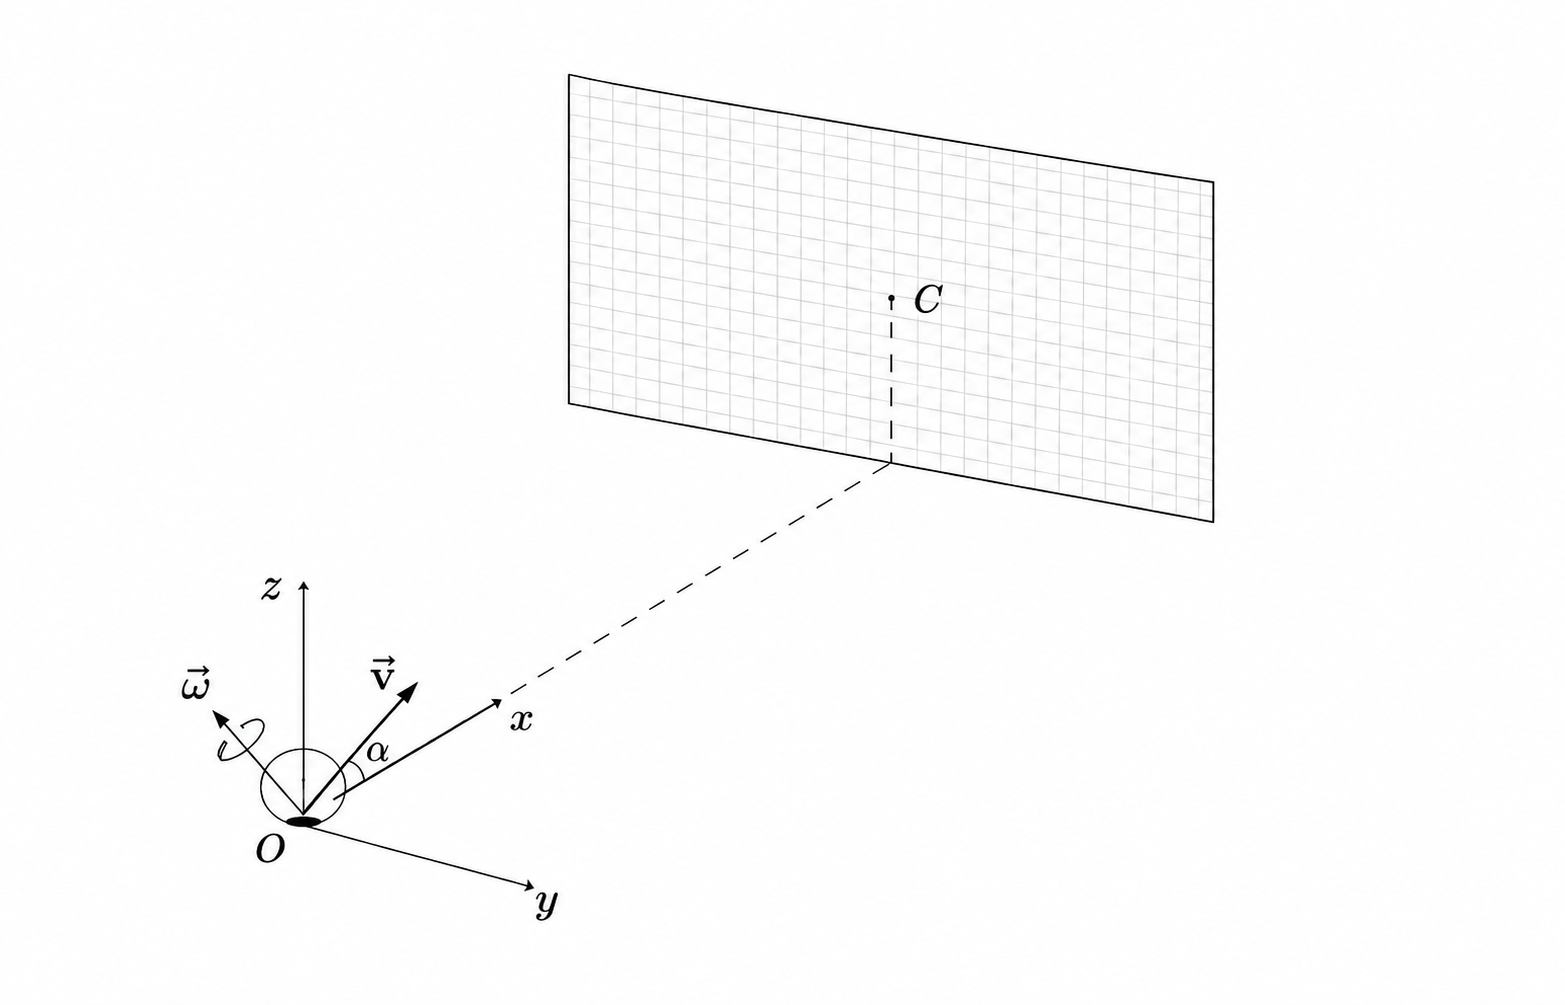
\includegraphics[width=0.78\textwidth]{penalty_geometry_new.png}
\caption{Penalty-kick geometry in local coordinates; $O$ is the nominal penalty mark and $C$ an illustrative goal-plane point.}\label{fig:geometry}\end{figure}
A clean opening crossing requires $|y|\le3.66-R$ and $R\le z\le2.44-R$. Descending centre height $z=R$ defines ground contact. Every model uses these same event definitions.

\subsection{Force Analysis}
\subsubsection{Gravity}
Gravity supplies a constant downward force,
\begin{equation}\boldsymbol F_g=-mg\boldsymbol e_z,\end{equation}
where $\boldsymbol e_z$ is the upward vertical unit vector. It produces downward curvature even when all aerodynamic forces are removed.

By Archimedes' principle the displaced air exerts an upward force on the ball. Its volume is $V_b=\frac43\pi R^3$, giving
\begin{equation}
\boldsymbol F_B=\rho V_b g\,\boldsymbol e_z
=\frac43\pi R^3\rho g\,\boldsymbol e_z.
\label{eq:buoyancy}\end{equation}
Together, gravity and buoyancy give $\boldsymbol F_g+\boldsymbol F_B=-(m-\rho V_b)g\boldsymbol e_z$. Buoyancy is $1.56\%$ of weight for the reference parameters. The baseline calculation uses gravity, drag and Magnus force, treating buoyancy as a small vertical correction.

Figure~\ref{fig:force-schematic} illustrates the relative airflow in the ball frame and the corresponding force directions. The right-hand example takes the spin axis out of the page; the lift direction follows the cross product.
\begin{figure}[H]\centering
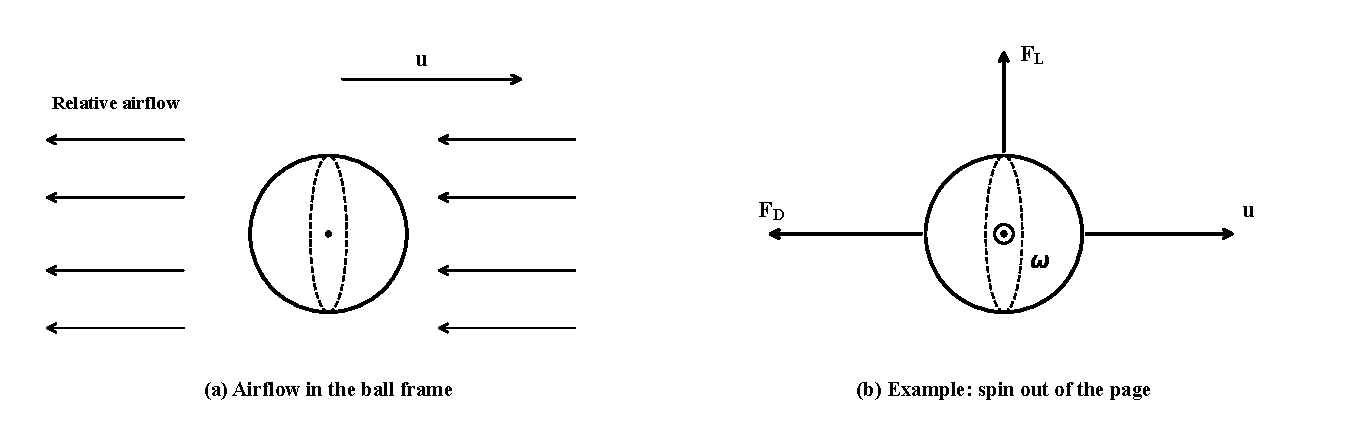
\includegraphics[width=.88\textwidth]{force_schematic.pdf}
\caption{Relative airflow and force directions. The symbol $\odot$ denotes spin out of the page; $\boldsymbol u$ in the left panel is the velocity of the ball relative to the air.}\label{fig:force-schematic}\end{figure}

\subsubsection{Aerodynamic Drag}\label{sec:drag}
With relative velocity $\boldsymbol u=\boldsymbol v-\boldsymbol v_{\rm wind}$, $u=\|\boldsymbol u\|$ and $A=\pi R^2$, drag is \cite{goff2009,kiratidis2018}
\begin{equation}\boldsymbol F_D=-\tfrac12\rho A C_D u\boldsymbol u.\label{eq:drag-force}\end{equation}
The drag coefficient $C_D$ is constant during each flight.
\subsubsection{Magnus Lift}\label{sec:lift}
\begin{figure}[H]\centering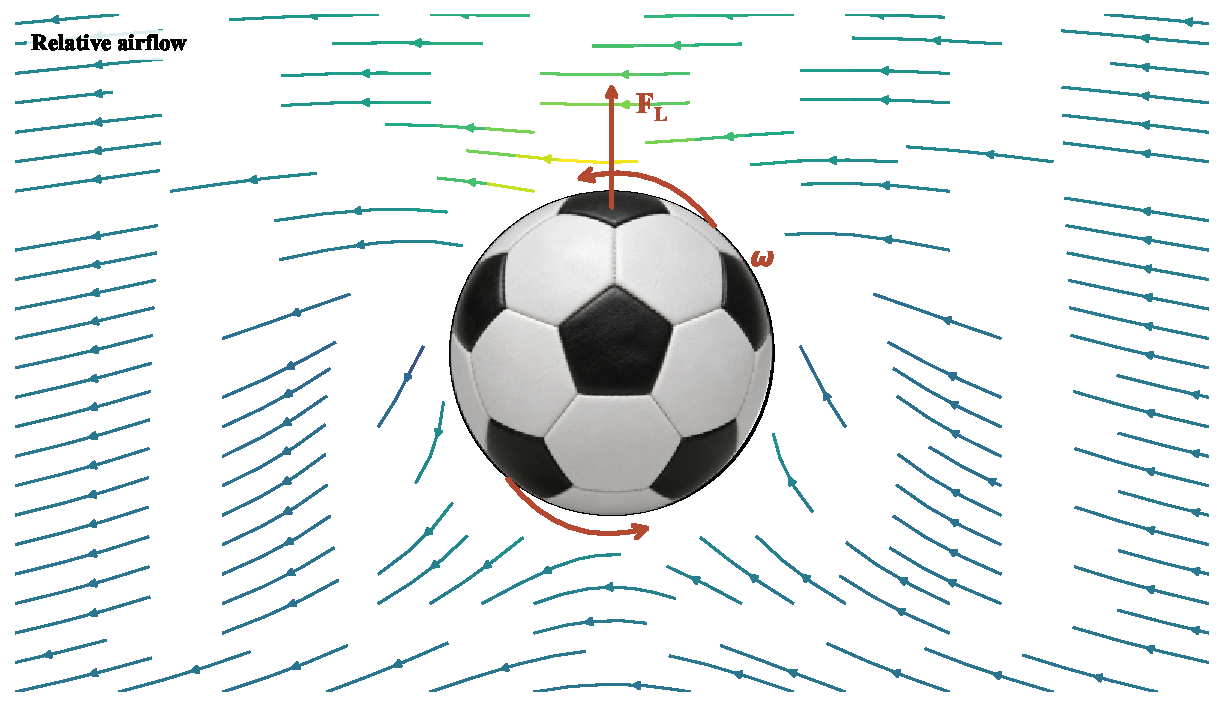
\includegraphics[width=.78\textwidth]{magnus_streamlines.pdf}\caption{Idealized flow around a spinning football.}\label{fig:magnus-flow}\end{figure}
Let $Re=2Ru/\nu$, $Sp=R\|\boldsymbol\omega\|/u$ and $C_L=\alpha Sp$. Resolving the transverse component yields
\begin{equation}\boldsymbol F_L=\tfrac12\rho A R\alpha(\boldsymbol\omega\times\boldsymbol u).\label{eq:lift-force}\end{equation}
The force vanishes at zero spin or zero relative velocity.
The forces on the football are summarized in the following diagram.
\begin{figure}[H]\centering
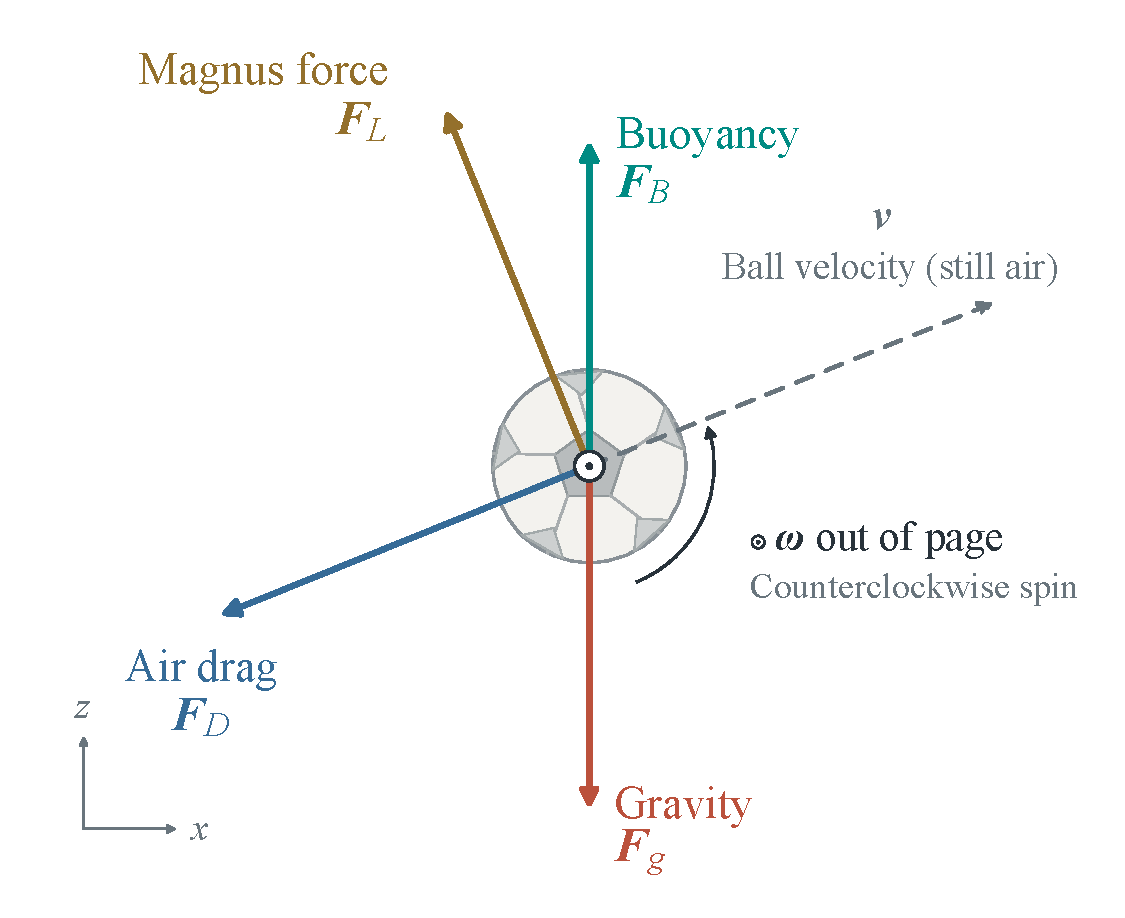
\includegraphics[width=.58\textwidth]{ball_force_diagram_times_xlarge.pdf}
\caption{Forces on the football: gravity, buoyancy, drag and Magnus force, with arrows showing their directions for the illustrated state.}\label{fig:ball-force-summary}\end{figure}

\subsection{Dynamical Equations}\label{sec:dynamics}
Newton's second law and angular-momentum balance give
\begin{equation}
m\dot{\boldsymbol v}=\sum\boldsymbol F,\qquad
\frac{d\boldsymbol L}{dt}=\boldsymbol Q,\qquad\boldsymbol L=I_b\boldsymbol\omega.
\end{equation}
With zero applied torque and constant spherical inertia, the main model is
\begin{equation}
\left\{\begin{aligned}
\dot{\boldsymbol r}&=\boldsymbol v,\\
m\dot{\boldsymbol v}&=\boldsymbol F_g+\boldsymbol F_D+\boldsymbol F_L,\\
\dot{\boldsymbol\omega}&=\boldsymbol0.
\end{aligned}\right.\label{eq:motion}
\end{equation}
Its initial conditions are
\begin{equation}
\left\{\begin{aligned}
\boldsymbol r(0)&=\boldsymbol r_0,\\
\boldsymbol v(0)&=(v_{x0},v_{y0},v_{z0}),\\
\boldsymbol\omega(0)&=(\omega_{x0},\omega_{y0},\omega_{z0}).
\end{aligned}\right.\label{eq:initial}
\end{equation}
The observed initial position fixes the origin of the flight. The six velocity and spin components determine its initial motion. In still air, drag removes mechanical energy while Magnus lift does no work along the velocity; gravity converts kinetic and potential energy during flight.





% BEGIN MODEL_SOLVING
\section{Model Solving}\label{sec:solving}
Early positions from three actual penalties determine inverse states whose continuations are compared with later observations. Two placement shots and one power shot provide different speeds, curvature directions and flight heights.
\begin{table}[H]\centering\small\caption{Four-model hierarchy and inverse quantities.}\label{tab:models}
\begin{tabular}{lll}\toprule
Model & Force or motion assumption & Inverse quantities\\\midrule
M1 & gravity & initial velocity (3)\\
M2 & gravity and drag & velocity and drag coefficient (4)\\
M3 & constant resultant force & velocity and acceleration (6)\\
M4 & gravity, drag and Magnus force & velocity, spin direction, $C_D$, $\alpha$ (7)\\\bottomrule
\end{tabular}\end{table}
The M3 resultant includes gravity and the other forces together. In M4, $C_D$ and $\alpha$ remain constant during a flight, while $C_L=\alpha Sp$ changes with speed. The references $C_D^*=\ReferenceCD$ and $\alpha^*=\ReferenceCL$ use $Re^*=333793$ and $Sp^*=0.19$, with $\alpha^*=C_L(Re^*,Sp^*)/Sp^*$ \cite{kiratidis2018}.

\subsection{Inverse Prediction from Three Real Penalties}\label{sec:inverse}
\subsubsection{Observations and numerical method}
The first selected position defines the time origin; the three inputs occur at $t=0,0.04,0.08$ s. The penalty mark is the horizontal origin, with $x$ towards the goal, $y$ lateral and $z$ the centre height. The goal plane is $x=11$ m. Data sources and source frames appear in \hyperref[app:data]{Appendix A}.

Integration uses DOP853 with a maximum step of 0.005 s, relative tolerance $10^{-10}$ and absolute tolerance $10^{-12}$. Forward roots of $x-11=0$ and descending roots of $z-R=0$ locate the goal crossing and first ground contact.

\subsubsection{Inversion and reference states}
M1 fits velocity, while M2 fits velocity and drag coefficient. M3 solves the three-position relation
\begin{equation}
\boldsymbol r(t)=\boldsymbol r_0+\boldsymbol v_0t+\tfrac12\boldsymbol a t^2.
\label{eq:m3-interpolation}\end{equation}
M4 fits three velocity components, two spin-direction angles and two coefficients by minimizing squared coordinate errors at the two later positions. Six deterministic starts are optimized and the smallest-residual result is selected; Table~\ref{tab:inverse-bounds} gives the ranges. Since $\alpha\boldsymbol\omega$ determines rotational deflection, we use a 30 rad/s reference magnitude and fit direction and $\alpha$.

Subsequent path and goal-plane errors are
\begin{equation}\begin{aligned}
\mathrm{RMSE}_{3D}&=\sqrt{\frac1n\sum_{i=1}^{n}\|\widehat{\boldsymbol r}(t_i)-\boldsymbol r_i\|^2},\\
E_g&=\sqrt{(\widehat y_g-y_g)^2+(\widehat z_g-z_g)^2}.
\end{aligned}\label{eq:prediction-errors}\end{equation}
Path comparisons use observations after the fitted times and before first contact or the goal crossing, with sample count $n$ listed in the table. $E_g$ is evaluated when a model crosses the goal plane; its observed counterpart comes from a source frame or interpolation between frames.

\subsection{Case Analysis and Validation}\label{sec:case-validation}
Figure~\ref{fig:shot-photos} illustrates the two shot styles.
\begin{figure}[H]\centering
\begin{subfigure}[t]{.48\textwidth}\centering
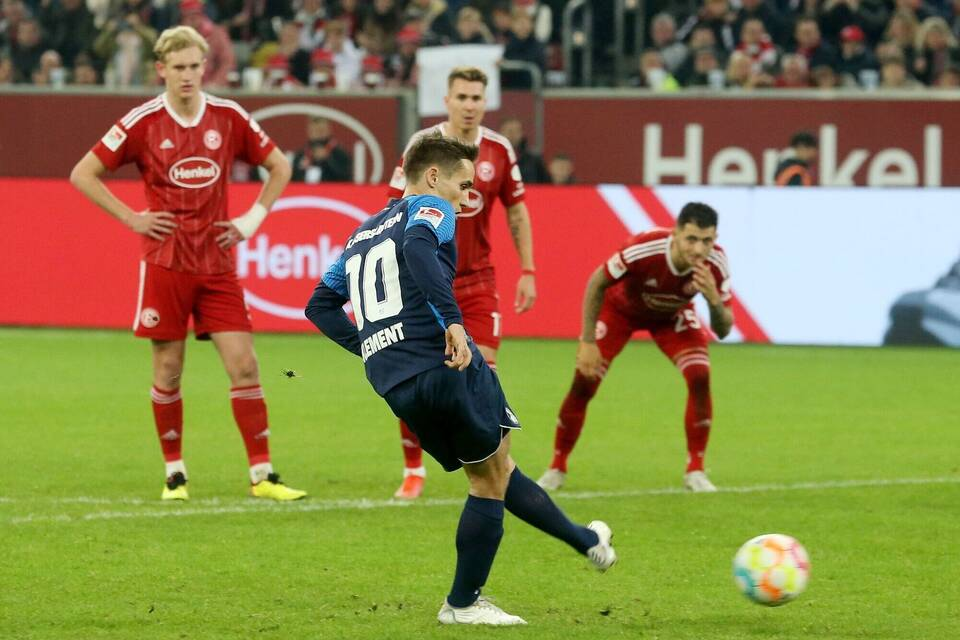
\includegraphics[width=\linewidth,height=.666667\linewidth]{placement_shot_example.png}
\caption{Illustrative placement shot.}\label{fig:placement-photo}
\end{subfigure}\hfill
\begin{subfigure}[t]{.48\textwidth}\centering
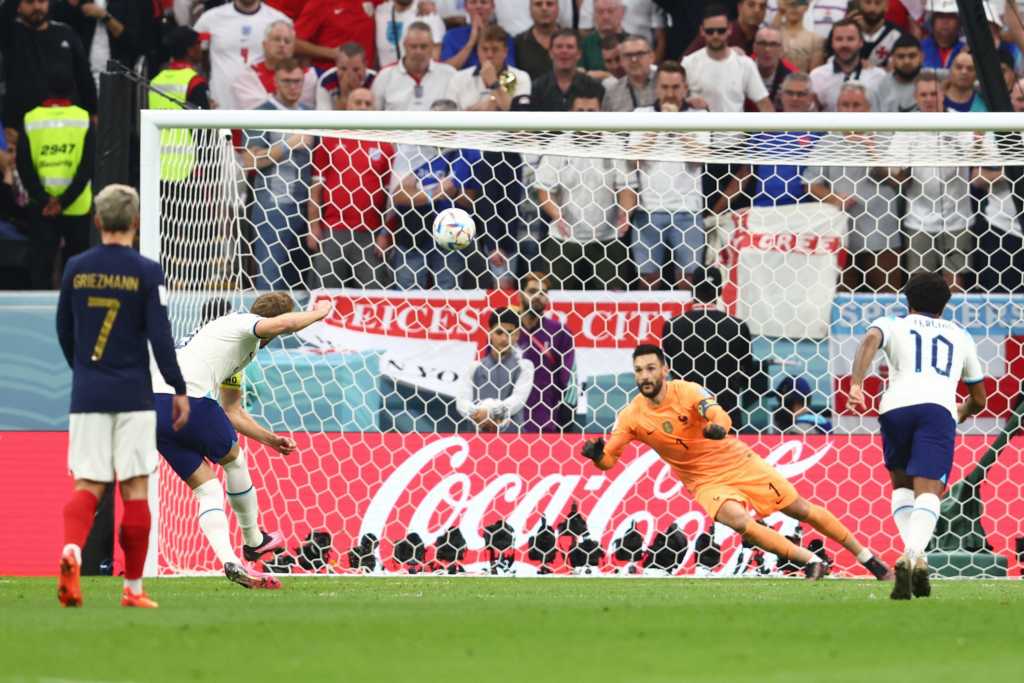
\includegraphics[width=\linewidth,height=.666667\linewidth]{power_shot_example.png}
\caption{Illustrative power shot.}\label{fig:power-photo}
\end{subfigure}
\caption{Photographic examples of placement and power shots.}\label{fig:shot-photos}
\end{figure}

Figure~\ref{fig:penalty-overview} summarizes the spatial paths. Open circles are inverse inputs, black points and lines are observations, coloured lines are predictions, and crosses are observed goal crossings.
\begin{figure}[H]\centering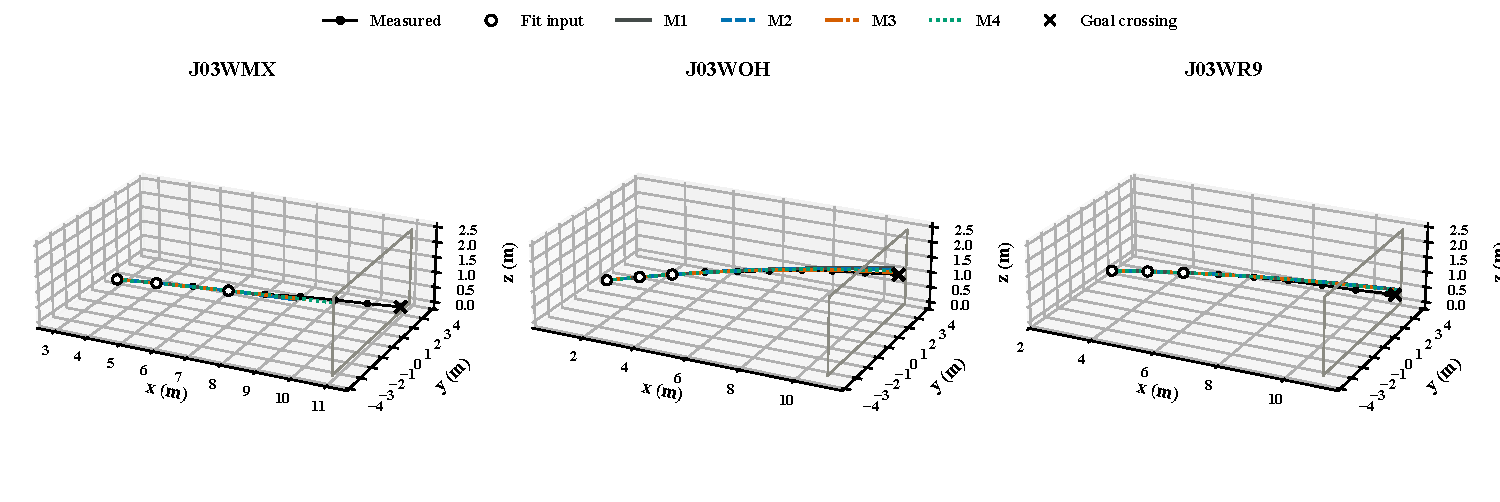
\includegraphics[width=\textwidth]{penalty_spatial_overview.pdf}
\caption{Observed and predicted paths for placement 1, the power shot and placement 2, from left to right. Fitting times are 0, 0.04 and 0.08 s in each case.}\label{fig:penalty-overview}\end{figure}

\subsubsection{Case 1: Placement shots}
\begin{figure}[H]\centering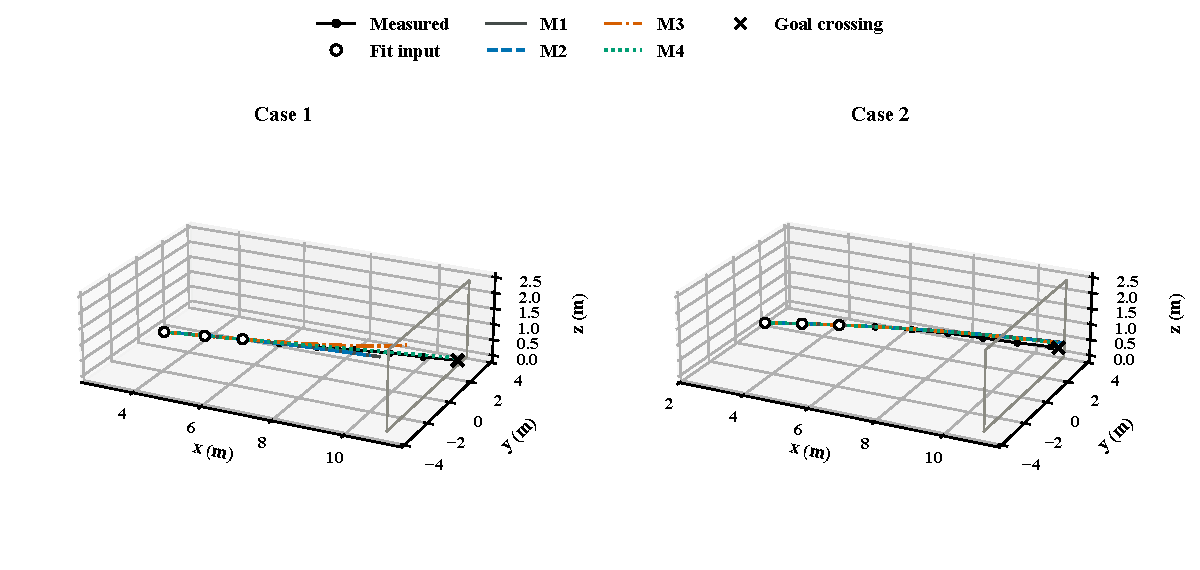
\includegraphics[width=.98\textwidth]{placement_spatial_comparison.pdf}
\caption{Measured and predicted trajectories for the two placement cases.}\label{fig:placement-paths}\label{fig:placement-example}\end{figure}
Both placement shots travel close to the ground. M4 gives starting speeds of \WMXSpeed\ m/s and \WRSpeed\ m/s. For placement 1, M1 and M2 reach the ground before the goal. M3 gives $a_x=-56.25$ m/s$^2$; Eq.~\eqref{eq:m3-interpolation} then gives a maximum $x=\WMXMThreeMaxX$ m, short of the goal. M4 reaches the plane with a crossing error of \WMXMFourGoalError\ m and a subsequent path RMSE of \WMXMFourPathRMSE\ m.

All four models reach the goal for placement 2, with crossing errors \WRMOneGoalError, \WRMTwoGoalError, \WRMThreeGoalError\ and \WRMFourGoalError\ m. Constant acceleration carries forward the early curvature in this case; M4 reduces the path RMSE from M3's \WRMThreePathRMSE\ m to \WRMFourPathRMSE\ m. Gravity draws a low flight downward, while the vertical Magnus component raises or lowers it according to spin direction. Together they determine whether the ball reaches the goal before contact.

\subsubsection{Case 2: Power shot}
M4 gives a starting speed of \WOHSpeed\ m/s. Figure~\ref{fig:penalty-J03WOH} displays the spatial path and coordinate histories.
\begin{figure}[H]\centering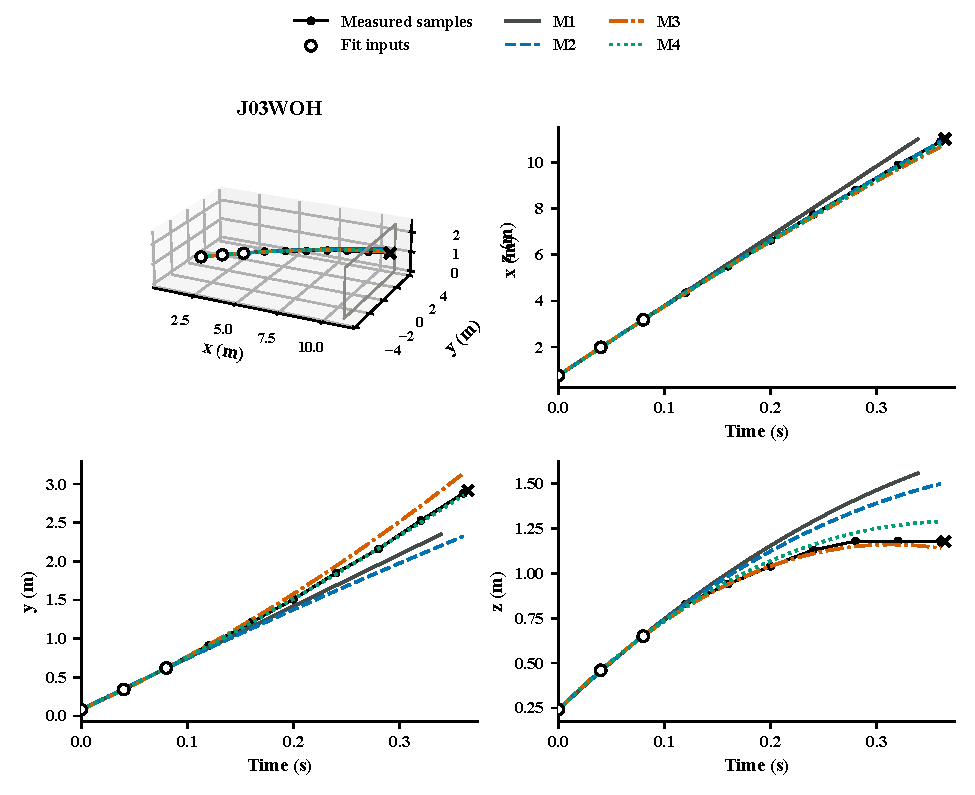
\includegraphics[width=\textwidth]{penalty_J03WOH.pdf}
\caption{Power-shot path and coordinate histories. Open circles are inverse inputs, black points are observations, and coloured curves are predictions.}\label{fig:power-paths}\label{fig:penalty-J03WOH}\end{figure}
M1--M4 have crossing errors of \WOHMOneGoalError, \WOHMTwoGoalError, \WOHMThreeGoalError\ and \WOHMFourGoalError\ m, and subsequent path RMSE values of \WOHMOnePathRMSE, \WOHMTwoPathRMSE, \WOHMThreePathRMSE\ and \WOHMFourPathRMSE\ m. Lateral motion in M1 and M2 follows the initial velocity; M3 extends constant acceleration. M4 curves the path through changing drag and Magnus forces, giving the smallest values of both errors for this shot.

\paragraph{Speed and aerodynamic forces.} Figure~\ref{fig:penalty-dynamics} gives the M4 speed and force histories. Initial drag is \WOHDrag\ N for the power shot and \WMXDrag\ N and \WRDrag\ N for the placement shots. Drag depends on $C_Dv^2$, combining speed with the fitted coefficient, and decreases as the flight slows. Linear lift depends on $\alpha(\boldsymbol\omega\times\boldsymbol v)$; the angle and direction between spin and velocity determine its lateral and vertical effects.
\begin{figure}[H]\centering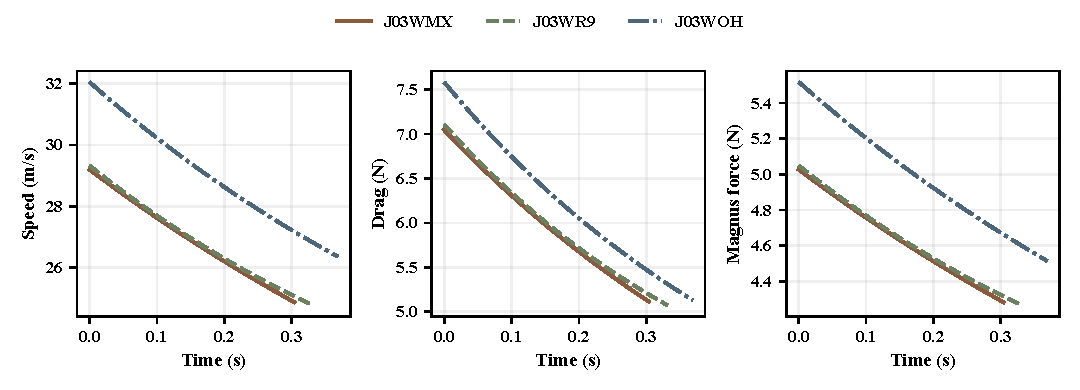
\includegraphics[width=\textwidth]{penalty_m4_dynamics.pdf}
\caption{M4 speeds, drag and Magnus force for the three penalties. Curves end at first ground contact or the goal plane.}\label{fig:penalty-dynamics}\end{figure}
\PenaltyErrorSummaryTable
% END MODEL_SOLVING


\section{Sensitivity Analysis}\label{sec:sensitivity}

% BEGIN SENSITIVITY_BODY
\noindent\hspace*{\parindent}This chapter uses the three early positions supplied in the problem to examine how initial motion, aerodynamic parameters and air density affect the goal-plane crossing and arrival time. The model includes gravity, drag and Magnus force, with still air, constant spin, a fixed mass of 0.43 kg and a fixed radius of 0.11 m.


\begin{table}[H]
\centering
\small
\renewcommand{\arraystretch}{1.16}
\caption{Early positions for the supplied example}
\begin{tabular}{lccc}
\toprule
Time $t$ (s) & $x$ (m) & $y$ (m) & $z$ (m)\\
\midrule
0 & 0 & 0 & 0.11\\
0.05 & 1.50 & 0.45 & 0.44\\
0.10 & 2.96 & 0.86 & 0.74\\
\bottomrule
\end{tabular}
\label{tab:sensitivity-reference}
\end{table}

Applying the inverse method of Section 4 with a reference spin magnitude of 30 rad/s gives the initial state


\begin{equation}
\begin{aligned}
\boldsymbol v_0&=(30.3784,\ 9.4074,\ 6.8974)\ \mathrm{m/s},\\
\boldsymbol\omega_0&=(19.7434,\ 1.2060,\ -22.5553)\ \mathrm{rad/s}.
\end{aligned}
\label{eq:sensitivity-reference-state}
\end{equation}

The corresponding drag coefficient is $C_D=0.3623$ and the linear lift parameter is $\alpha=2.2877$. The maximum early-coordinate residual is 0.784 mm. The trajectory reaches the goal plane at $t_g^*=0.398967$ s, with crossing coordinates $(y_g^*,z_g^*)=(2.6159,1.9526)$ m.


Taking this trajectory as the reference, we first vary individual parameters to identify their effects on position and arrival time. We then retain the early-position constraints and examine predictions from different parameter combinations. Finally, joint perturbations provide the crossing distribution and its statistical ranges.


\FloatBarrier
\subsection{Effects of Individual Parameters on Crossing Position and Arrival Time}\label{sec:sensitivity-local}

\noindent\hspace*{\parindent}Each parameter is varied separately while the others remain at their reference values. Table~\ref{tab:sensitivity-scan-ranges} lists the nine perturbation ranges: percentages denote changes relative to the reference value, and direction angles vary about their reference orientation. Each parameter takes 41 equally spaced values, giving 369 trajectories.

\begin{table}[H]\centering\small
\renewcommand{\arraystretch}{1.15}
\caption{Perturbation ranges for the nine parameters}
\begin{tabular}{lc}\toprule
Parameter & Perturbation range\\\midrule
Launch speed & $\pm$5\%\\
Velocity azimuth & $\pm$$2^\circ$\\
Velocity elevation & $\pm$$2^\circ$\\
Spin magnitude & $\pm$10\%\\
Spin-axis azimuth & $\pm$$2^\circ$\\
Spin-axis elevation & $\pm$$2^\circ$\\
Drag coefficient & $\pm$10\%\\
Lift parameter & $\pm$10\%\\
Air density & $\pm$10\%\\
\bottomrule\end{tabular}\label{tab:sensitivity-scan-ranges}
\end{table}


\Needspace{5\baselineskip}
The changes in crossing coordinates and arrival time relative to the reference trajectory are defined as


\begin{equation}
\begin{aligned}
\Delta y_g&=y_g-y_g^*,\qquad
\Delta z_g=z_g-z_g^*,\qquad
\Delta t_g=t_g-t_g^*,\\
D_g&=\sqrt{(\Delta y_g)^2+(\Delta z_g)^2}.
\end{aligned}
\label{eq:sensitivity-displacement}
\end{equation}

Figures~\ref{fig:sensitivity-one-position} and~\ref{fig:sensitivity-one-time} show the crossing-position and arrival-time responses. Table~\ref{tab:sensitivity-one-factor} takes direction perturbations of $\pm1^\circ$ and other perturbations of $\pm5\%$ from these scans, reporting the larger displacement and absolute time change from each positive--negative pair.


\begin{table}[H]
\centering
\small
\renewcommand{\arraystretch}{1.16}
\caption{One-parameter effects on goal-plane crossing and arrival time}
\begin{tabular}{lccc}
\toprule
Parameter & Perturbation & Maximum $D_g$ (cm) & Maximum $\lvert\Delta t_g\rvert$ (ms)\\
\midrule
Launch speed & $\pm$5\% & 8.356 & 20.659\\
Velocity azimuth & $\pm$$1^\circ$ & 20.070 & 1.965\\
Velocity elevation & $\pm$$1^\circ$ & 20.218 & 1.692\\
Spin magnitude & $\pm$5\% & 3.873 & 0.287\\
Spin-axis azimuth & $\pm$$1^\circ$ & 1.002 & 0.071\\
Spin-axis elevation & $\pm$$1^\circ$ & 0.852 & 0.084\\
Drag coefficient & $\pm$5\% & 0.620 & 2.274\\
Lift parameter & $\pm$5\% & 3.873 & 0.287\\
Air density & $\pm$5\% & 4.142 & 1.990\\
\bottomrule
\end{tabular}
\label{tab:sensitivity-one-factor}
\end{table}

For the perturbation sizes in Table~\ref{tab:sensitivity-one-factor}, initial direction primarily affects crossing position: a $1^\circ$ change in azimuth or elevation moves the crossing by about 0.20 m. Speed strongly affects arrival time; a $\pm5\%$ change produces a maximum time difference of 20.659 ms and a maximum crossing displacement of 8.356 cm. Direction directly determines lateral and vertical motion, while speed changes the time to the goal and therefore the accumulated effects of gravity and aerodynamic forces.


The responses to spin magnitude and the lift parameter coincide because the linear Magnus force is proportional to the product $\alpha\boldsymbol\omega$. The same relative change in either spin magnitude or $\alpha$ produces the same force and trajectory response. Scaling them inversely gives


\begin{equation}
\boldsymbol\omega_0'=k\boldsymbol\omega_0,\qquad
\alpha'=\alpha/k
\quad\Longrightarrow\quad
\boldsymbol F_L'=\boldsymbol F_L,\qquad k>0.
\label{eq:sensitivity-spin-compensation}
\end{equation}

Different spin magnitudes and lift parameters can therefore produce the same trajectory. Spin-axis orientation affects the magnitude and direction of deflection through $\boldsymbol\omega\times\boldsymbol v$. Air density scales both drag and Magnus force, changing deceleration and curvature together.


\begin{figure}[!htbp]
\centering
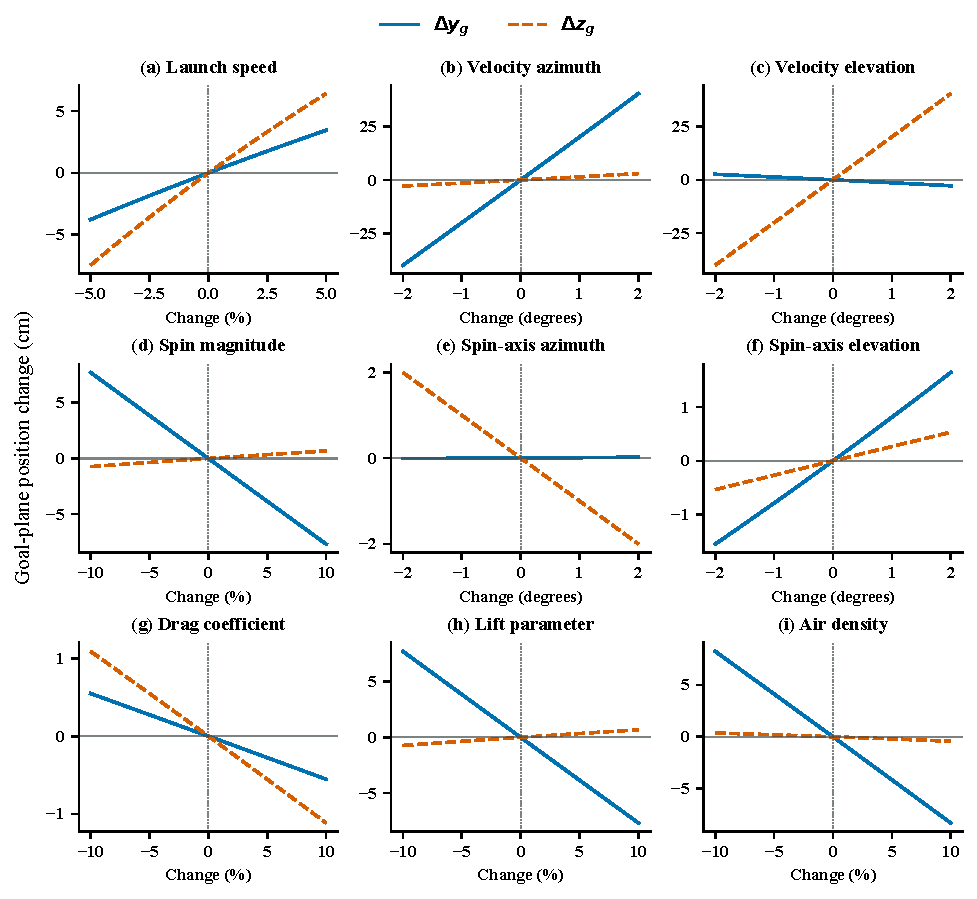
\includegraphics[clip,width=\textwidth]{one_factor_position_response.pdf}
\caption{Goal-plane coordinate responses to nine one-parameter perturbations. Blue solid curves show $\Delta y_g$ and orange dashed curves show $\Delta z_g$, in cm. Vertical scales differ between panels.}
\label{fig:sensitivity-one-position}
\end{figure}


\begin{figure}[!htbp]
\centering
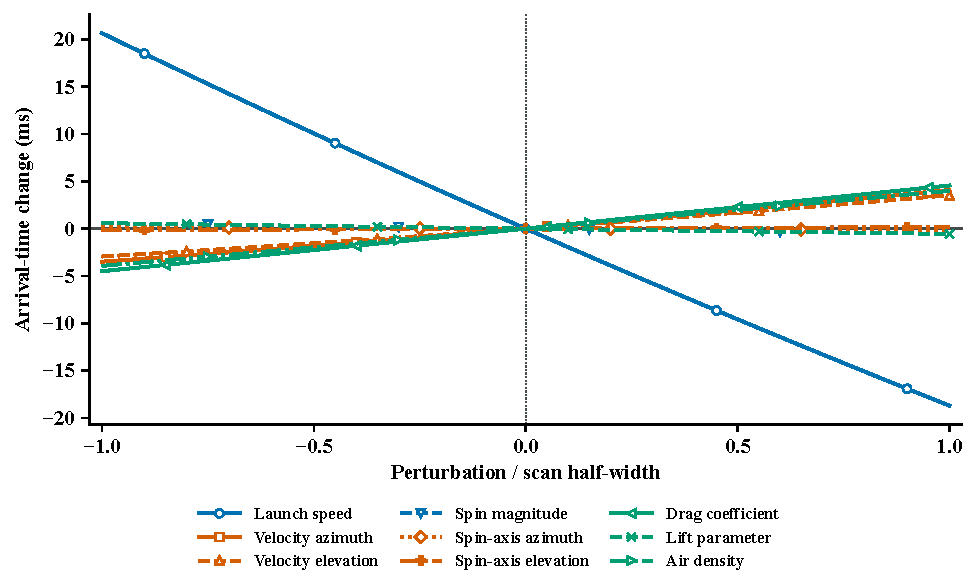
\includegraphics[clip,width=\textwidth]{one_factor_time_response.pdf}
\caption{Arrival-time responses. Perturbation divided by scan half-width is plotted horizontally, so $\pm1$ denotes each scan endpoint. The vertical axis is $\Delta t_g$ (ms); positive values mean later arrival.}
\label{fig:sensitivity-one-time}
\end{figure}


\FloatBarrier
\subsection{Prediction Differences under Early-Position Constraints}\label{sec:sensitivity-constrained}

\noindent\hspace*{\parindent}The preceding analysis varies one parameter while holding the others fixed. We now examine how much the goal-plane crossing can change when different parameter combinations reproduce the same early positions approximately.


Using the aerodynamic reference values $C_D^*$ and $\alpha^*$ from Section 4, define


\begin{equation}
\lambda_D=C_D/C_D^*,\qquad
\lambda_\alpha=\alpha/\alpha^*.
\label{eq:sensitivity-coefficient-ratios}
\end{equation}

Each coefficient multiplier takes 17 equally spaced values in $[1.2,1.8]$, forming $17\times17$ combinations. For each combination, the initial spin component $\omega_{x0}$ takes 33 equally spaced values in $[-60,60]$ rad/s. The three initial velocity components and the other two spin components are then fitted to the early positions in Table~\ref{tab:sensitivity-reference}. The constraints are a total speed not exceeding 35 m/s, an absolute value not exceeding 60 rad/s for each spin component, and a maximum early-coordinate residual not exceeding 2 mm.


The supplementary search yields 5049 compatible trajectories across 153 aerodynamic-parameter combinations. Restricting both multipliers to $[1.35,1.65]$, corresponding to $\pm10\%$ changes in each aerodynamic parameter about its reference-trajectory value, gives 2079 trajectories across 63 combinations. Table~\ref{tab:sensitivity-profile} lists their crossing and arrival-time ranges, and Figure~\ref{fig:sensitivity-constrained} shows their crossing positions.


\begin{table}[H]
\centering
\small
\renewcommand{\arraystretch}{1.16}
\caption{Goal-plane crossing ranges under early-position constraints}
\begin{tabular}{lccc}
\toprule
Range of each multiplier & $y_g$ (m) & $z_g$ (m) & $t_g$ (s)\\
\midrule
$[1.35,1.65]$ & 2.5538--2.6550 & 1.9061--2.0369 & 0.3972--0.4025\\
$[1.2,1.8]$ & 2.5478--2.6601 & 1.8972--2.0430 & 0.3972--0.4043\\
\bottomrule
\end{tabular}
\label{tab:sensitivity-profile}
\end{table}

\Needspace{5\baselineskip}

Within the wider parameter range, the largest crossing displacement among the searched trajectories is 0.1074 m relative to the reference. The minimum-residual solutions for each aerodynamic-parameter combination lie at the spin-component bounds; plotting these solutions alone produces two clusters. Intermediate spin states satisfying the same 2 mm position constraint form the band joining the clusters in Figure~\ref{fig:sensitivity-constrained}. Thus, initial velocity and spin can compensate for aerodynamic changes over the early observation interval, while different force histories accumulate into distinct subsequent crossings.


\begin{figure}[!htbp]
\centering
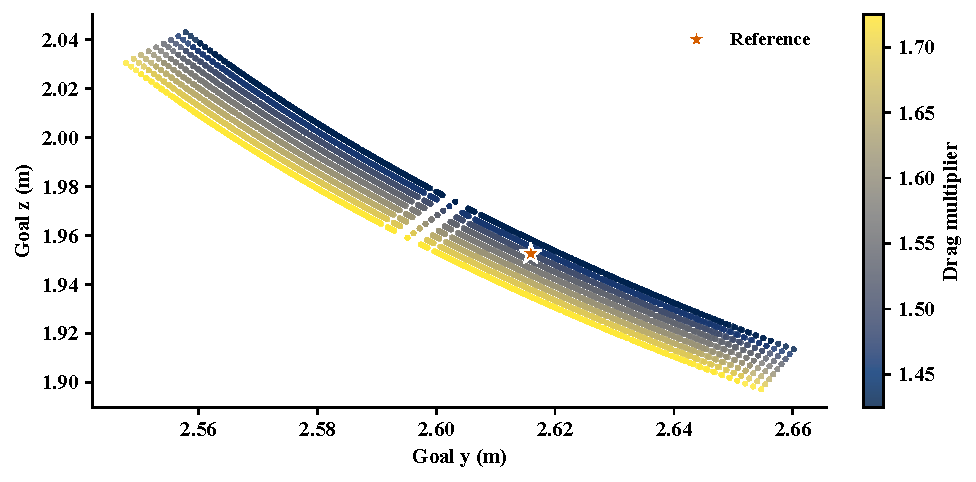
\includegraphics[clip,width=.88\textwidth]{conditional_crossings.pdf}
\caption{The 5049 crossings from the supplementary search under the 2 mm early-position constraint. Colour denotes $\lambda_D$; the orange star marks the reference trajectory.}
\label{fig:sensitivity-constrained}
\end{figure}


\FloatBarrier
\subsection{Crossing Distribution under Joint Perturbations}\label{sec:sensitivity-mc}

\noindent\hspace*{\parindent}To examine simultaneous changes in several conditions, the nine parameters are sampled independently and uniformly over the ranges in Section 5.1, producing 100000 inputs. Mass, radius and initial position remain fixed. Integrating the equations for each input gives the crossing distribution under jointly varying launch conditions and aerodynamic parameters.


\begin{table}[H]
\centering
\small
\renewcommand{\arraystretch}{1.16}
\caption{Crossings and arrival times for 100000 jointly perturbed trajectories}
\begin{tabular}{lcc}
\toprule
Output & Sample minimum--maximum & Central 95\% interval, one coordinate\\
\midrule
$y_g$ (m) & 1.9633--3.2143 & 2.1858--3.0505\\
$z_g$ (m) & 1.4381--2.4646 & 1.5534--2.3535\\
$t_g$ (s) & 0.3685--0.4346 & 0.3783--0.4218\\
\bottomrule
\end{tabular}
\label{tab:sensitivity-mc}
\end{table}

The central 95\% intervals in Table~\ref{tab:sensitivity-mc} use the 2.5th and 97.5th percentiles of each output. The mean crossing is $(2.6170,1.9511)$ m, with lateral and vertical standard deviations of 0.2455 m and 0.2360 m. The largest displacement from the reference crossing is 0.801 m.


To describe lateral and vertical variation jointly, write $\boldsymbol q_i=(y_{g,i},z_{g,i})^{\mathsf T}$ and use the sample mean $\bar{\boldsymbol q}$ and covariance matrix $\widehat\Sigma$ to define


\begin{equation}
d_i^2=(\boldsymbol q_i-\bar{\boldsymbol q})^{\mathsf T}
\widehat\Sigma^{-1}(\boldsymbol q_i-\bar{\boldsymbol q}).
\label{eq:sensitivity-standardized-distance}
\end{equation}

\Needspace{5\baselineskip}

Taking the empirical 95th percentile $c_{0.95}=4.5916$ of $d_i^2$ gives the joint region


\begin{equation}
\mathcal E_{0.95}=\left\{\boldsymbol q:
(\boldsymbol q-\bar{\boldsymbol q})^{\mathsf T}\widehat\Sigma^{-1}
(\boldsymbol q-\bar{\boldsymbol q})\le c_{0.95}\right\}.
\label{eq:sensitivity-joint-region}
\end{equation}

The set $\mathcal E_{0.95}$ is the ellipse boundary and its interior in Figure~\ref{fig:sensitivity-mc}. The ellipse line marks the boundary, and the region contains 95\% of the simulated crossings. The goal is 2.44 m high; accounting for the 0.11 m ball radius requires a centre height between 0.11 and 2.33 m and a lateral position satisfying $|y_g|\le3.55$ m for the whole ball to pass through. By these criteria, 95772 trajectories clear the opening, or 95.772\%; the other 4228 trajectories, or 4.228\%, exceed the 2.33 m centre-height limit.


\begin{figure}[!htbp]
\centering
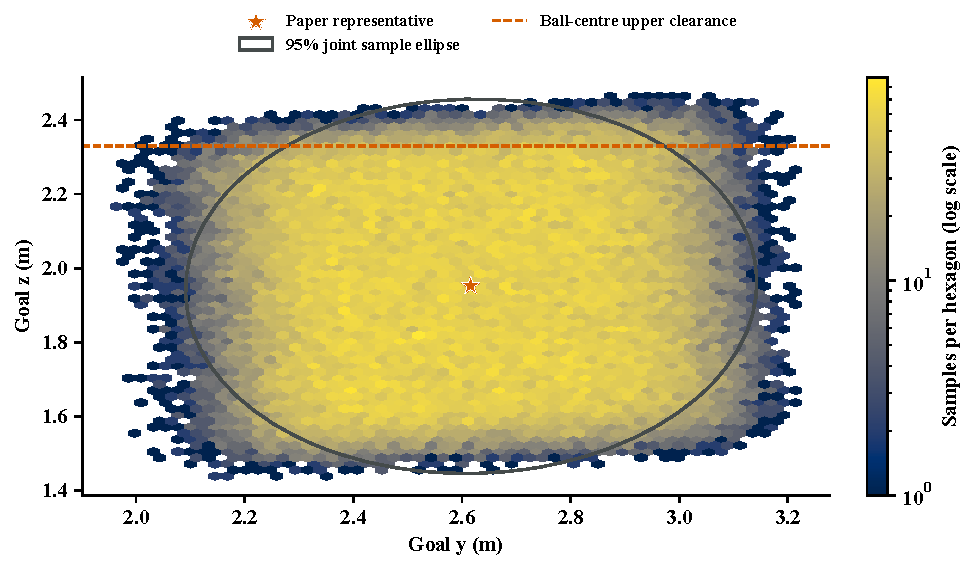
\includegraphics[clip,width=\textwidth]{monte_carlo_crossings.pdf}
\caption{Goal-plane crossings under 100000 joint perturbations. Hexagon colour indicates sample count, the ellipse denotes the joint 95\% region, and the dashed line marks the ball-centre height limit $z_g=2.33$ m.}
\label{fig:sensitivity-mc}
\end{figure}


Figure~\ref{fig:sensitivity-mc-parallel} displays 400 randomly selected trajectories, linking the nine inputs to crossing coordinates and arrival time. Inputs are scaled to 0--1 using their perturbation bounds; outputs use the extrema of the full 100000-trajectory sample. The subset contains 385 blue lines for trajectories clearing the goal and 15 orange lines for trajectories crossing too high. Each line connects one set of launch conditions and aerodynamic parameters to its predicted outcome.


\begin{figure}[!htbp]
\centering
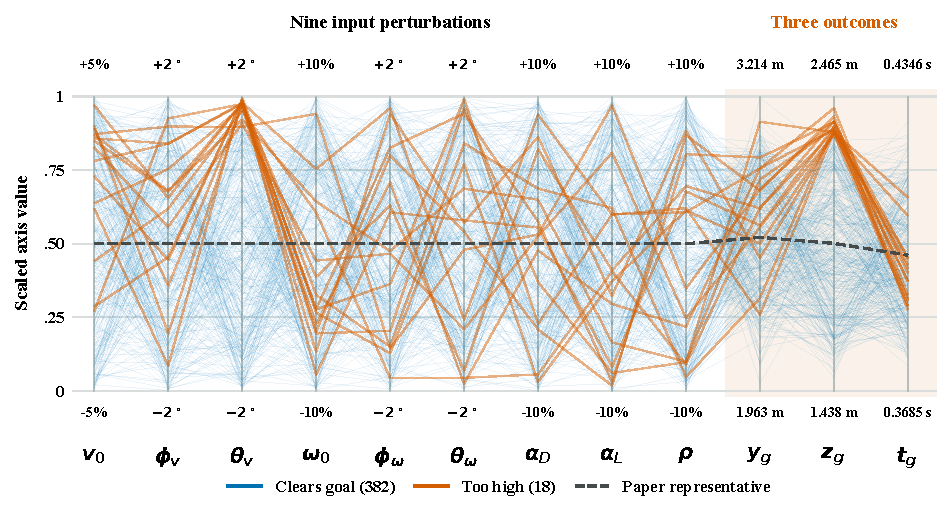
\includegraphics[clip,width=\textwidth]{monte_carlo_parallel_coordinates.pdf}
\caption{Parallel coordinates linking perturbed inputs, crossing coordinates and arrival time. The first nine axes are inputs and the last three are outputs. The displayed subset contains 385 trajectories clearing the opening and 15 crossing too high.}
\label{fig:sensitivity-mc-parallel}
\end{figure}


Figure~\ref{fig:sensitivity-mc-convergence} checks whether the crossing statistics stabilize as the number of simulations increases, informing the choice of 100000 samples for estimating the central 95\% intervals. The blue sample extrema expand as additional extreme trajectories appear, while the orange percentile intervals gradually stabilize. Increasing the sample from 50000 to 100000 changes the lateral and vertical interval endpoints by at most 0.264 mm and 0.506 mm, and the arrival-time endpoints by at most 0.138 ms. Two additional runs of 10000 trajectories with independent random seeds differ from the main sample by at most 5.425 mm laterally, 4.320 mm vertically and 0.328 ms in time. These comparisons show that further sampling has a small effect on the central-interval estimates.


\begin{figure}[!htbp]
\centering
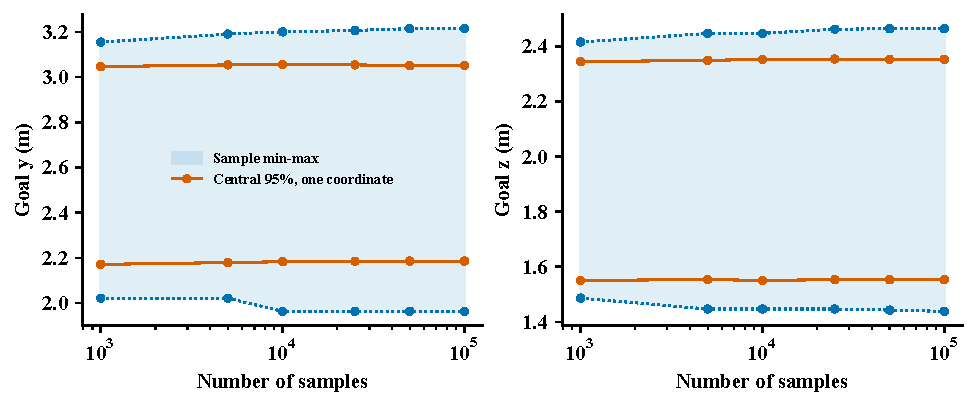
\includegraphics[clip,width=\textwidth]{monte_carlo_convergence.pdf}
\caption{Convergence of crossing statistics with simulation sample size. Blue shading and dotted curves show sample extrema; orange curves show each coordinate's central 95\% interval, illustrating the stability of interval estimates as sample size increases.}
\label{fig:sensitivity-mc-convergence}
\end{figure}

\FloatBarrier
% END SENSITIVITY_BODY


\section{Discussion of Other Factors}\label{sec:other}
The main model isolates gravity, drag and Magnus lift. We now examine the physical effects omitted from its geometry, spin evolution and ambient airflow.
\subsection{Asymmetric Surface Geometry}\label{sec:surface}
A full-flight simulation compares realistic football geometry with a smooth sphere \cite{paudel}. For launch speeds of 10, 15 and 20 m/s and spin rates of 31.5, 63 and 94.5 rad/s, their results show that seams and surface structure alter separation, wake dynamics and Magnus force. The smooth sphere produces greater lateral bending in their nine comparisons, and vertical flight-time differences become more visible at higher speed and rotation.

\begin{figure}[H]\centering
\begin{subfigure}[t]{.40\textwidth}\centering
\begin{minipage}[c][3.5in][c]{\linewidth}\centering
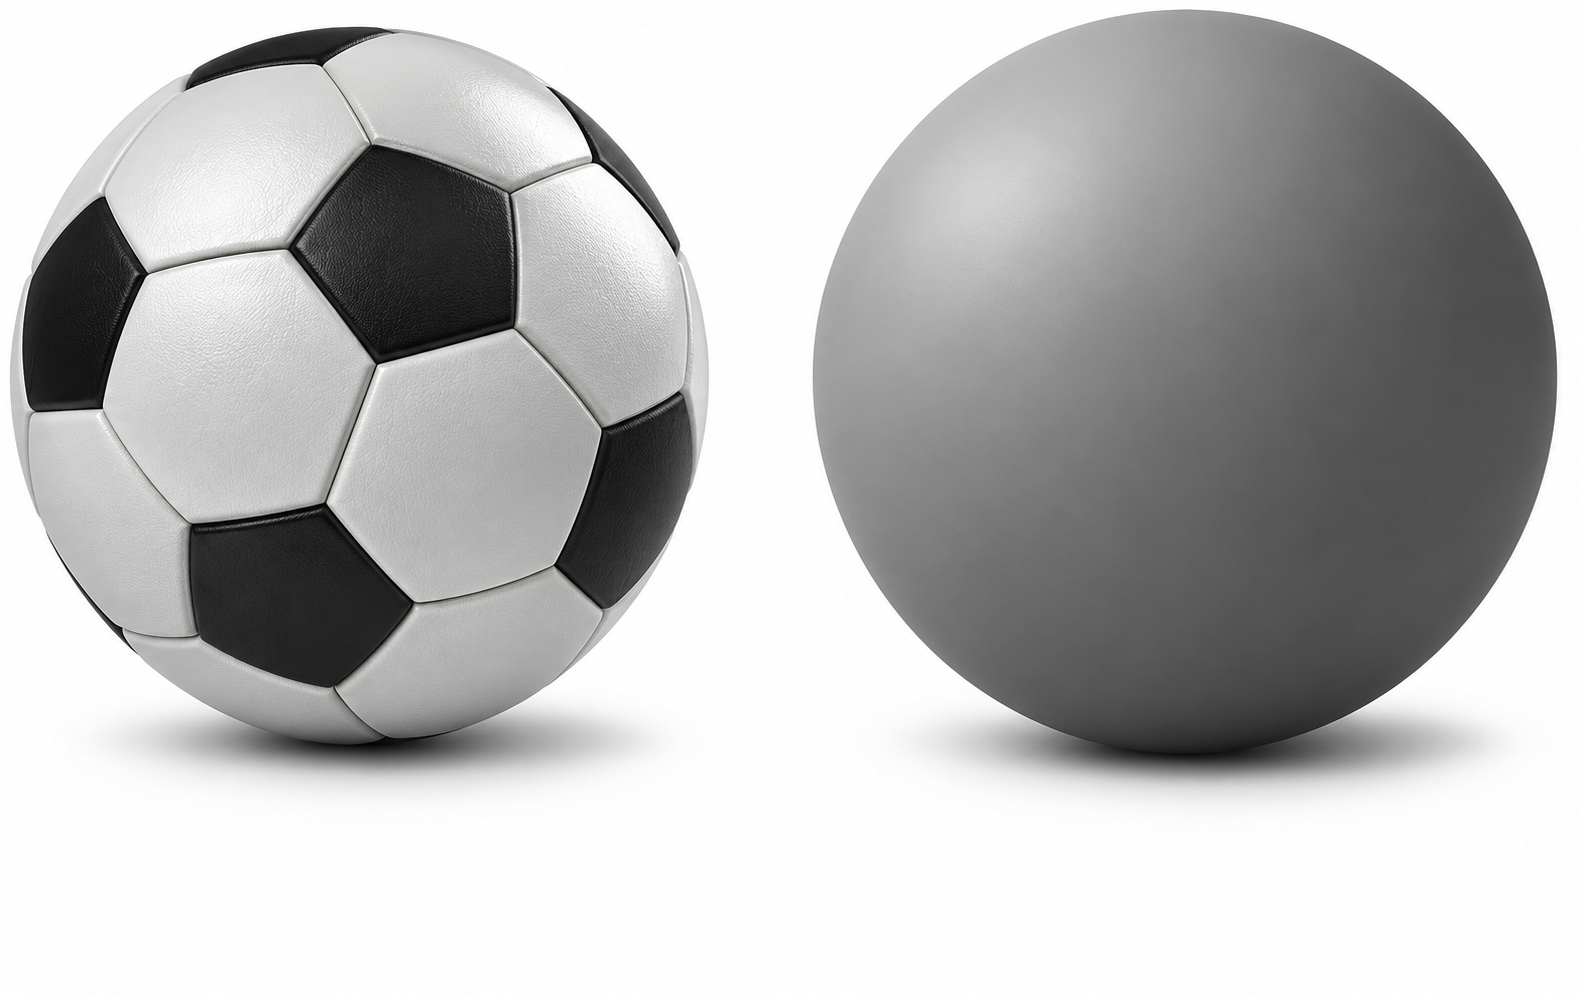
\includegraphics[width=\linewidth]{surface_comparison.png}
\end{minipage}
\caption{Illustrative seamed-football and smooth-sphere comparison \cite{paudel}.}\label{fig:surface-geometry}
\end{subfigure}\hfill
\begin{subfigure}[t]{.57\textwidth}\centering
\begin{minipage}[c][3.5in][c]{\linewidth}\centering
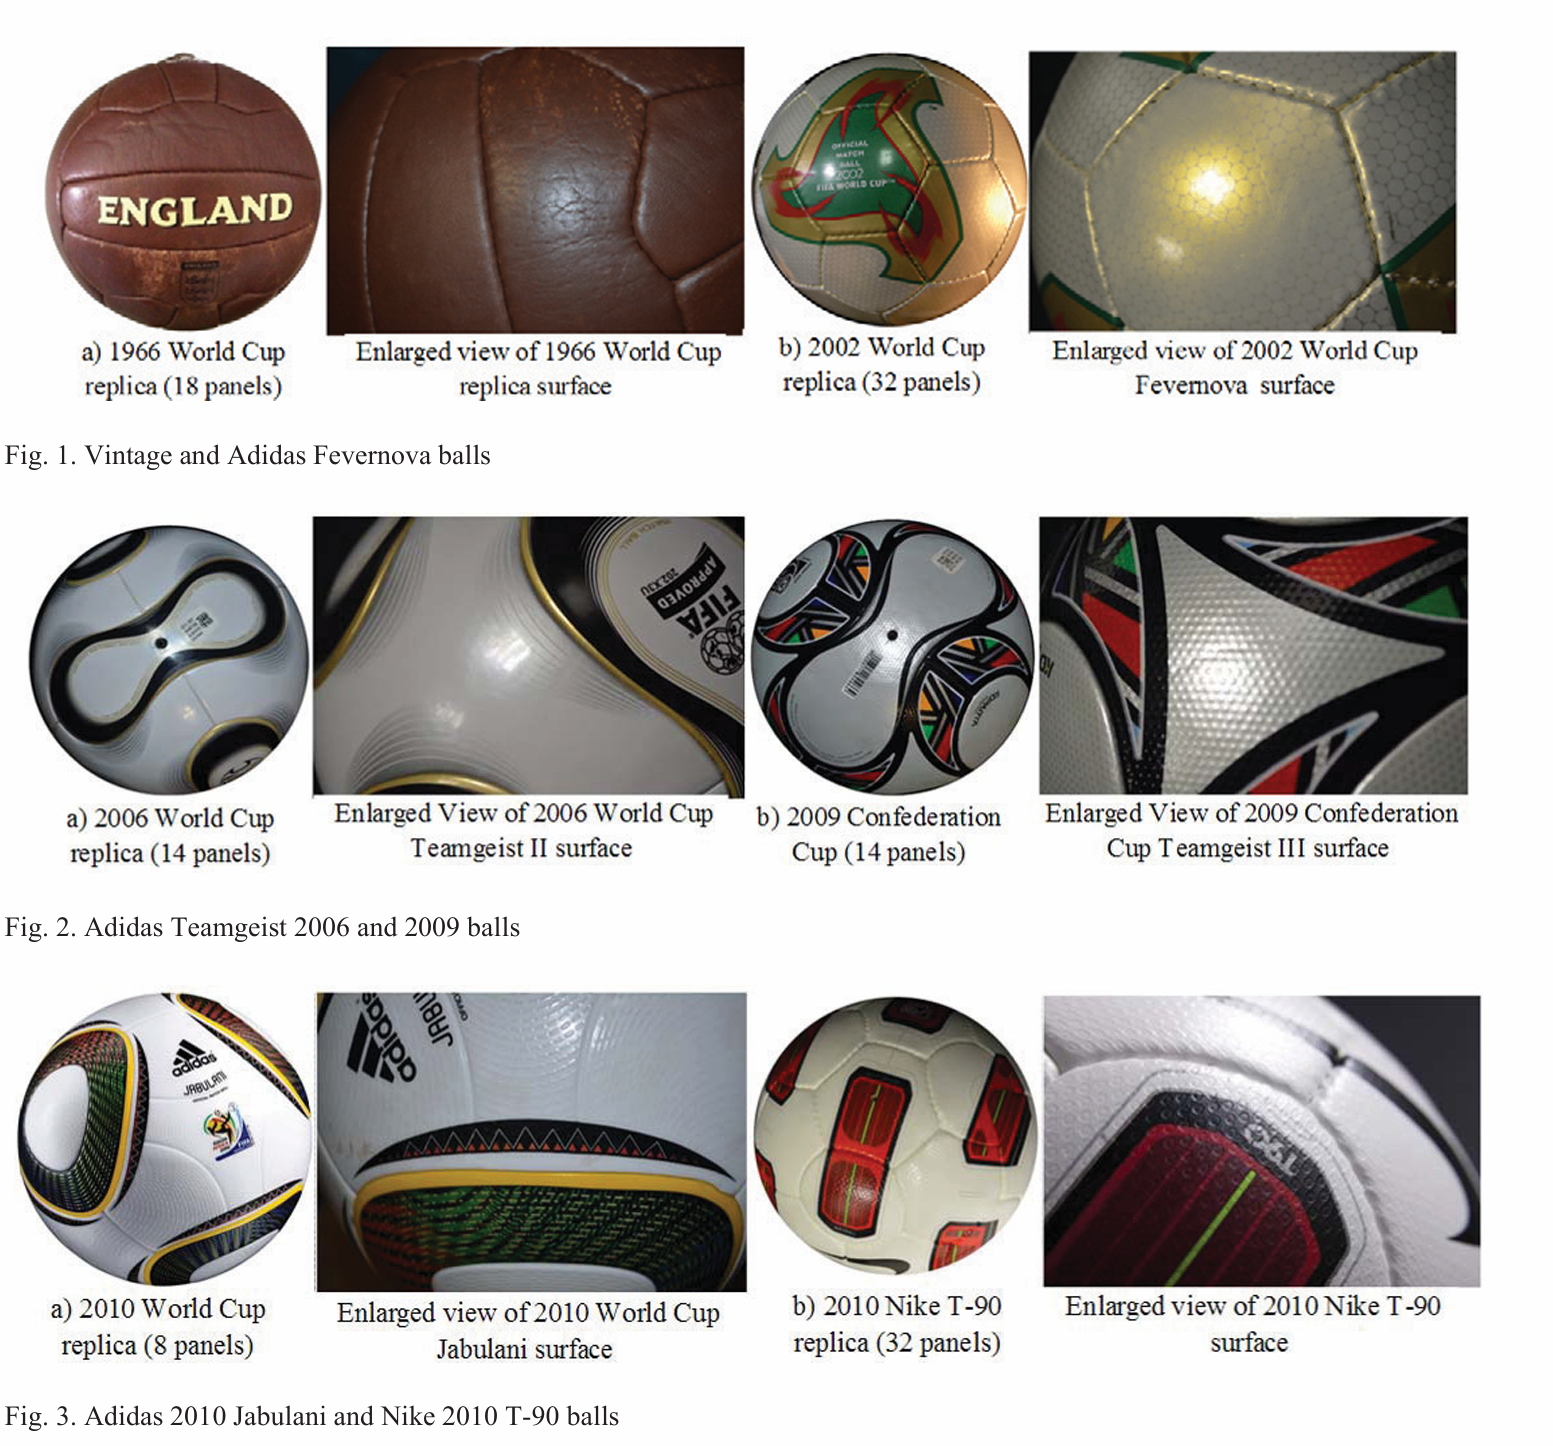
\includegraphics[width=\linewidth]{alam_ball_surfaces.png}
\end{minipage}
\caption{Six footballs and surface details, reproduced from Figures 1--3 of Alam et al.\ \cite{alam2012}.}\label{fig:alam-surfaces}
\end{subfigure}
\caption{Football geometry, panels and surface textures.}\label{fig:surface-details}
\end{figure}

Wind-tunnel experiments measured drag coefficients over a range of Reynolds numbers for six footballs and a smooth sphere \cite{alam2012}. Figure~\ref{fig:alam-surfaces} shows the panels and surface textures of these footballs, while Figure~\ref{fig:alam-drag} compares their drag coefficients. The differences illustrate the influence of ball surface structure on aerodynamic drag.


\begin{figure}[H]\centering
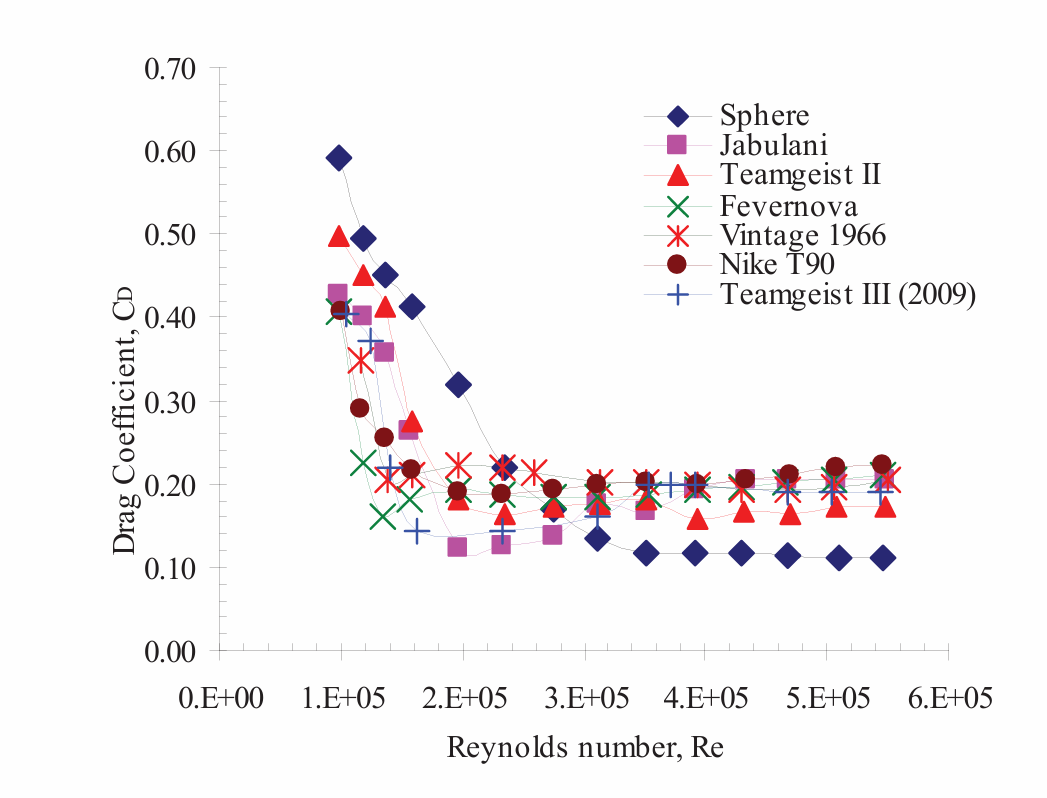
\includegraphics[width=.76\textwidth]{alam_drag_comparison.png}
\caption{Drag coefficient against Reynolds number for different footballs and a smooth sphere, reproduced from Figure 5 of the source\cite{alam2012}.}\label{fig:alam-drag}\end{figure}

The spherical geometry in the present report describes the centre-of-mass motion and projected area. Its force coefficients come from football measurements, so the average surface influence enters through $C_D$ and $C_L$. Explicit panel orientation and asymmetric wake fluctuations provide a further level of description when lateral-force details are important. These published results support retaining football-specific coefficients in a spherical trajectory model.

\subsection{Rotation and Aerodynamic Damping}\label{sec:rotation}
Aerodynamic torque opposes spin, gradually weakening rotation and changing the Magnus force. We use the high-Reynolds-number rotational-damping model described by Grad et al.\ and MuJoCo \cite{grad2026,mujoco381}, in which stronger spin produces stronger resistance. The angular-drag parameter is the software reference value $C_{\rm angular}=1.5$, with the thin-shell inertia approximation \cite{maponi}. Viscous damping is much weaker than the inertial contribution in this example, so the comparison focuses on the latter.

The reference curved shot has initial velocity $(\CurvedVX,0,\CurvedVZ)$ m/s, spin $(0,0,35)$ rad/s and unit force corrections. Holding this state fixed, we and compare constant spin with rotational damping. Figure~\ref{fig:torque} shows both the spin evolution and the resulting trajectory difference.
\begin{figure}[H]\centering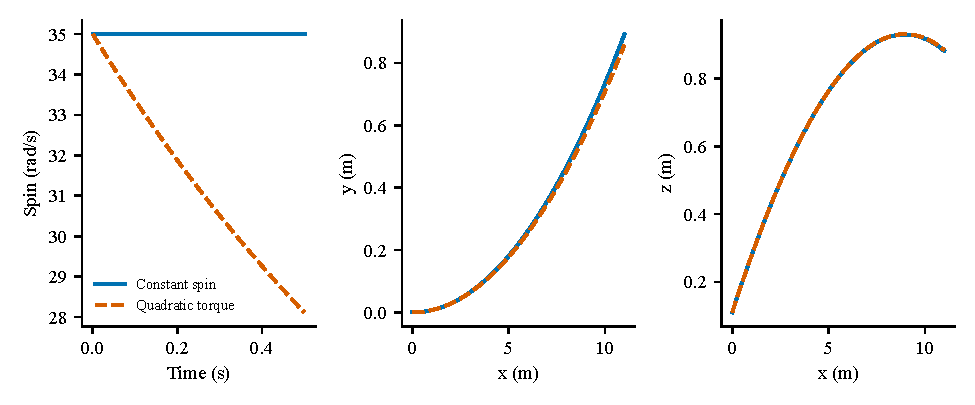
\includegraphics[width=\textwidth]{torque_comparison.pdf}
\caption{Constant spin and rotational damping under the same initial curved-shot conditions.}\label{fig:torque}\end{figure}
\TorqueResults

\subsection{Wind Speed and Force Estimates}\label{sec:wind}
Wind changes the airflow through $\boldsymbol u=\boldsymbol v-\boldsymbol v_{\rm wind}$ \cite{maponi}. At fixed coefficients, a wind speed $w$ along the flight direction changes the dynamic-pressure scale by
\begin{equation}
\frac{q_{\rm head}}{q_0}=(1+w/v)^2,\qquad
\frac{q_{\rm tail}}{q_0}=(1-w/v)^2,\qquad
\frac{q_{\rm cross}}{q_0}=1+(w/v)^2.
\end{equation}
Crosswind rotates the airflow by $\arctan(w/v)$ and changes the force direction. Table~\ref{tab:wind} evaluates 1, 3 and 5 m/s winds at the 24 m/s curved-shot speed.
For the M4 linear lift law, Eq.~\eqref{eq:lift-force} also gives the headwind and tailwind effects along the flight direction. With fixed spin and $0\le w<v$,
\begin{equation}
\frac{F_{L,\mathrm{head}}}{F_{L,0}}=1+\frac wv,\qquad
\frac{F_{L,\mathrm{tail}}}{F_{L,0}}=1-\frac wv.
\label{eq:wind-linear-lift}\end{equation}
\WindResultsTable
A 5\% limit on the headwind dynamic-pressure change corresponds to $w/v\leq\sqrt{1.05}-1$, or $w\leq\WindThreshold$ m/s at this launch. The still-air approximation is most suitable for indoor or weak-wind flight; stronger wind should enter through the relative-velocity calculation.

\section{Conclusions}
The four models describe gravitational fall, deceleration, a constant resultant force and rotational deflection. M3 obtains constant acceleration from three positions. M4 inserts constant $C_D$ and $C_L=\alpha Sp$ into the motion equations, updating drag and Magnus force as speed changes.

M4 gives crossing errors of \WMXMFourGoalError, \WRMFourGoalError\ and \WOHMFourGoalError\ m for the three penalties. Its power-shot crossing error and subsequent path RMSE are the smallest among the four models. For placement 1, M3 passes through the early positions but reaches a maximum $x=\WMXMThreeMaxX$ m, short of the goal; M4 supplies a goal-plane prediction for this low flight.

In the competition-position example, a $1^\circ$ launch-direction change moves the crossing by about 0.20 m, while speed strongly affects arrival time. Spin magnitude and $\alpha$ compensate through the linear lift law. The largest grid-search shift under the 2 mm position constraint is \SensitivityConditionalShift\ m; \MCClearPercent\% of 100,000 jointly perturbed flights clear the opening.

Rotational damping shifts the reference curved-shot crossing by \TorqueDisplacement\ m. Wind enters through relative velocity: along the flight direction, drag changes with the squared speed ratio and linear Magnus force with the speed ratio.

\section{Model Evaluation}

\subsection{Model Strengths}

\noindent\hspace*{\parindent}\textbf{Connecting forces and trajectory changes.} The model incorporates gravitational fall, drag-induced deceleration and rotational deflection in a common equation of motion, relating trajectory curvature to changes in force magnitude and direction. The four-model comparison shows how different force descriptions and the constant-acceleration approximation affect predictions, providing a physical interpretation of the differences between low placement shots and higher power shots.

\textbf{Connecting early inference and later validation.} Three early positions are used to estimate initial motion and relevant parameters, after which the corresponding equations predict the subsequent trajectory. Later measured positions provide comparisons of the path and goal-plane crossing, connecting early fitting with subsequent predictive validation. Shared coordinates and definitions of ground contact and goal-plane crossing also make results comparable across models and shot cases.

\textbf{Reference predictions and crossing ranges.} Individual-parameter scans distinguish the effects on crossing position and arrival time. The position-constrained search reveals differences in predictions from parameter combinations matching the early observations, while joint perturbations give crossing distributions over specified ranges. Together, these analyses connect parameter changes to the final prediction, describing a reference crossing, response trends and distribution ranges.

\Needspace{18\baselineskip}
\subsection{Model Weaknesses}

\noindent\hspace*{\parindent}\textbf{Coupling of initial motion and aerodynamic parameters.} Over a short observation interval, initial velocity, spin and aerodynamic parameters can compensate for one another, allowing initially similar trajectories to separate later in flight. In the linear lift relation, spin magnitude and the lift parameter enter the force through their product, so different parameter values can also generate the same trajectory. Additional early tracking positions and direct spin measurements would further constrain initial motion and aerodynamic parameters.

\textbf{Simplified aerodynamics and environmental conditions.} The main model treats the drag coefficient and linear lift parameter as constants during each flight and assumes still air and constant spin. Flow transitions, ball orientation and wake fluctuations alter aerodynamic forces, while wind and rotational damping affect relative airflow and spin evolution. More detailed descriptions require aerodynamic data for each ball type, together with wind and spin measurements.

\textbf{Limited coverage of measured conditions.} The measured comparison covers two placement shots and one power shot. Tracking records spanning additional ball types, shot techniques and wind conditions would allow assessment across more operating conditions. Joint perturbations use independent uniform sampling of nine parameters; estimating their distributions and correlations from measurements would bring the simulated crossing distribution closer to actual shooting conditions.

\addcontentsline{toc}{section}{References}
\begin{thebibliography}{99}
\raggedright
\bibitem{kamp2018} J. van der Kamp, M. Dicks, J. A. Navia and B. No\"el, ``Goalkeeping in the soccer penalty kick,'' \emph{German Journal of Exercise and Sport Research}, 48, 169--175, 2018. \url{https://doi.org/10.1007/s12662-018-0506-3}.
\bibitem{hunter2018} A. H. Hunter, S. C. Murphy, M. J. Angilletta Jr. and R. S. Wilson, ``Anticipating the direction of soccer penalty shots depends on the speed and technique of the kick,'' \emph{Sports}, 6, 73, 2018. \url{https://doi.org/10.3390/sports6030073}.
\bibitem{griffiths2005} I. Griffiths, C. Evans and N. Griffiths, ``Tracking the flight of a spinning football in three dimensions,'' \emph{Measurement Science and Technology}, 16, 2056--2065, 2005. \url{https://doi.org/10.1088/0957-0233/16/10/022}.
\bibitem{goff2017} J. E. Goff, J. Kelley, C. M. Hobson, K. Seo, T. Asai and S. B. Choppin, ``Creating drag and lift curves from soccer trajectories,'' \emph{European Journal of Physics}, 38, 044003, 2017. \url{https://doi.org/10.1088/1361-6404/aa6fcd}.
\bibitem{bray} K. Bray and D. G. Kerwin, ``Modelling the flight of a soccer ball in a direct free kick,'' \emph{Journal of Sports Sciences}, 21, 75--85, 2003. \url{https://doi.org/10.1080/0264041031000070994}.
\bibitem{bassek} M. Bassek, R. Rein, H. Weber and D. Memmert, ``An integrated dataset of spatiotemporal and event data in elite soccer,'' \emph{Scientific Data}, 12, 195, 2025. \url{https://doi.org/10.1038/s41597-025-04505-y}.
\bibitem{dataset} DFL, ``Sportec Open DFL Dataset,'' CC BY 4.0. Official release: \url{https://doi.org/10.6084/m9.figshare.28196177}. Data mirror: \url{https://huggingface.co/datasets/pysport/idsse-data}.
\bibitem{maponi} P. Maponi and R. Piombin, ``A computational framework to predict the soccer ball trajectory,'' \emph{Journal of Applied Mathematics}, 2025, 7425581. \url{https://doi.org/10.1155/jama/7425581}.
\bibitem{paudel} S. Paudel and J. Yan, ``High-fidelity simulations of full-flight soccer ball aerodynamics using a monolithic overset approach,'' \emph{Computational Mechanics}, 77, 1245--1265, 2026. \url{https://doi.org/10.1007/s00466-025-02705-2}.
\bibitem{myers} T. G. Myers and S. L. Mitchell, ``A mathematical analysis of the motion of an in-flight soccer ball,'' \emph{Sports Engineering}, 16, 29--41, 2013. \url{https://doi.org/10.1007/s12283-012-0105-8}.
\bibitem{asai2007} T. Asai, K. Seo, O. Kobayashi and R. Sakashita, ``Fundamental aerodynamics of the soccer ball,'' \emph{Sports Engineering}, 10, 101--110, 2007. \url{https://doi.org/10.1007/BF02844207}.
\bibitem{kiratidis2018} A. L. Kiratidis and D. B. Leinweber, ``An aerodynamic analysis of recent FIFA World Cup balls,'' \emph{European Journal of Physics}, 39, 034001, 2018. \url{https://doi.org/10.1088/1361-6404/aaa888}. Equations and parameters: \url{https://arxiv.org/abs/1710.02784v2}.
\bibitem{grad2026} \L{}. Grad, K. M. Czajkowski and A. Varashylau, ``Physics-Based 3D Ball Trajectory Reconstruction from Monocular Soccer Video: A Multi-Model Benchmark,'' \emph{Proceedings of the IEEE/CVF Conference on Computer Vision and Pattern Recognition Workshops}, 9940--9948, 2026. \href{https://openaccess.thecvf.com/content/CVPR2026W/CVsports/supplemental/Grad_Physics-Based_3D_Ball_CVPRW_2026_supplemental.pdf}{Supplementary material}, Section~8.4.
\bibitem{mujoco381} MuJoCo developers, MuJoCo 3.8.1, ellipsoid fluid model, \texttt{mj\_viscousForces} in \texttt{src/engine/engine\_passive.c}. \href{https://github.com/google-deepmind/mujoco/blob/3.8.1/src/engine/engine_passive.c}{Version 3.8.1 source}; default angular drag: \href{https://mujoco.readthedocs.io/en/stable/XMLreference.html#body-geom-fluidcoef}{XML reference, geom/fluidcoef}. Accessed 8 November 2026.
\bibitem{goff2009} J. E. Goff and M. J. Carr\'e, ``Trajectory analysis of a soccer ball,'' \emph{American Journal of Physics}, 77, 1020--1027, 2009. \url{https://doi.org/10.1119/1.3197187}.
\bibitem{alam2012} F. Alam, H. Chowdhury, M. Stemmer, Z. Wang and J. Yang, ``Effects of surface structure on soccer ball aerodynamics,'' \emph{Procedia Engineering}, 34, 146--151, 2012. \url{https://doi.org/10.1016/j.proeng.2012.04.026}.
\end{thebibliography}

\newpage\section*{Appendix A: Data Sources, Frame Selection and Parameter Bounds}\label{app:data}
\addcontentsline{toc}{section}{Appendix A: Data Sources, Frame Selection and Parameter Bounds}
\begingroup\def\small{\fontsize{10}{11}\selectfont}\small\setlength{\intextsep}{3pt}\captionsetup{font=small,skip=3pt}\renewcommand{\arraystretch}{.95}
The three penalties come from the Sportec Open DFL dataset, which associates match events with TRACAB Gen5 multi-camera tracking at 25 Hz\cite{bassek,dataset}. The supplied CSV retains 39 source frames, with 15, 12 and 12 frames for the three events.
\begin{table}[H]\centering\small\caption{Correspondence between case labels and source records}\label{tab:data-provenance}
\begin{tabular}{llll}\toprule
Case & Event ID & Player & Selected samples\\\midrule
Placement 1 & J03WMX & Dejan Ljubicic & 3, 4, 5\\
Placement 2 & J03WR9 & Philipp Klement & 3, 4, 5\\
Power shot & J03WOH & Dawid Igor Kownacki & 2, 3, 4\\\bottomrule
\end{tabular}\end{table}
The first selected position is the time origin and the fitting times are 0, 0.04 and 0.08 s. Their source-time origins are 0.08, 0.08 and 0.04 s in the table's order. Repeated and post-goal records are retained; later positions are used only for validation. The observed goal crossing uses a source frame or interpolation. The height field is interpreted in metres as ball-centre height, and coordinates are converted with $x=X-41.5$, $y=Y$ and $z=Z_{\rm original}$.

Table~\ref{tab:penalty-observations} gives the early inputs and goal crossings; Table~\ref{tab:inverse-bounds} gives the inversion ranges.
\PenaltyObservationTable
\InverseBoundsTable
Table~\ref{tab:m4-parameters} gives the fitted M4 parameters, with $\boldsymbol n=\boldsymbol\omega/30$.
\MFourParameterTable

\endgroup
\newpage\addcontentsline{toc}{section}{Reproduction Code}
\section*{Reproduction Code}
The project contains the original penalty CSV, coordinate conversion, shared inversion, prediction results and figure scripts. The excerpts show the common state equation and force evaluation. Paper and program use the same coefficients and bounds; computation, plotting and bilingual table generation are separate commands.
\begin{lstlisting}[language=Python]
def state_derivative(t, state, config):
    """The single nine-state RHS used for prediction and inverse fitting."""
    f = forces(state[3:6], state[6:9], config)
    return np.r_[state[3:6], sum(f.values())/config.mass,
                 rotational_torque(state[6:9], config)/config.moment_of_inertia]
\end{lstlisting}
\begin{lstlisting}[language=Python]
def forces(velocity, spin, config):
    """Return force components on ball, in newtons."""
    v = np.asarray(velocity, dtype=float) - np.asarray(config.wind, dtype=float)
    omega = np.asarray(spin, dtype=float)
    speed = np.linalg.norm(v)
    weight = (config.mass * np.asarray(config.constant_acceleration, dtype=float)
              if config.constant_acceleration is not None else
              np.array([0., 0., -config.mass * config.gravity if config.use_gravity else 0.]))
    drag = np.zeros(3)
    magnus = np.zeros(3)
    if speed > 1e-12:
        cd, cl, _, _, _ = coefficients(velocity, spin, config)
        q_area = 0.5 * config.air_density * np.pi * config.radius**2 * speed**2
        if config.use_drag:
            drag = -q_area * config.drag_scale * cd * v / speed
        cross = np.cross(omega, v)
        norm = np.linalg.norm(cross)
        if config.use_magnus and norm > 1e-12:
            # The literature fit is for transverse spin. Project its effect
            # onto the plane perpendicular to airflow for an oblique spin axis.
            sin_angle = norm / (np.linalg.norm(omega) * speed)
            magnus = q_area * config.lift_scale * cl * sin_angle * cross / norm
    return {"gravity": weight, "drag": drag, "magnus": magnus}
\end{lstlisting}
\end{document}
